\cleardoublepage%
\chapter{\label{chap:Experiment}Experimental Setup}%
\noindent The theories within the Standard Model, along with any other theories aimed at explaining unresolved phenomena, must undergo experimental testing. The close cooperation between comprehending the processes in particle physics and conducting experimental tests is an important aspect of this field of science. This chapter provides a brief introduction to the experimental setup utilized for the results presented in this thesis.\\
\indent In Section \ref{sec:exp_LHC} the LHC layout and its performance during the data taking periods are presented. The CMS detector layout and its subsystem technologies are highlighted in Section \ref{sec:exp_CMS}. Finally, in Section \ref{sec:exp_CMS_8} a brief overview of the muon trigger performance for the start of 2024 data-taking period is presented as part of the work done for this thesis. 

\section{\label{sec:exp_LHC}Large Hadron Collider}
\noindent The LHC is the largest and most powerful particle accelerator ever built, operating at the European Organization for Nuclear Research (CERN\footnote{Conseil Européen pour la Recherche Nucléaire}) laboratory, near Geneva, Switzerland \cite{Brüning:782076, Lyndon_Evans_2008}. It has a circumference of 26.7 km and is built in the same tunnel that previously housed the Large Electron Positron (LEP) Collider. It is located between 45 and 170 metres below ground level and has a slight slope of 1.23\% towards Lake Geneva. The LHC was designed to collide two high energy proton beams with a maximum center of mass energy of 14 TeV \footnote{The maximum operating energy of the LHC so far is $\sqrt{s} = 13.6$ TeV \cite{cern}}. Additionally, it facilitates collisions of heavy ion beams across a spectrum of atomic numbers, reaching energies up to 5 TeV per nucleon.\\
\indent The machine consists of two parallel rings hosting counter-rotating proton beams that are accelerated to nearly the speed of light and collide at the 4 interaction points. There are multiple magnets in different sizes and varieties, aiming at keeping the beams in circular orbit, focusing and squeezing them before collision. More specifically there are 1232 dipole magnets 15 m in length which bend the beams and 392 quadrupole magnets, each 5–7 m long, which focus the beams.  There are also higher order magnets (hexapoles, octapoles) which correct and compress the beam just before the interaction in order to increase the collision probability. All magnets are superconducting, i.e. they have almost zero electrical resistance so that they can accept high current intensities and thus generate a magnetic field of more than 8 T. However, in order to achieve the superconductivity of the magnets, it is  required to be cooled to very low temperatures, $-271.3^{\circ}$C, which is only possible using superfluid helium \cite{CERN_cooling}.
\subsection{\label{sec:exp_LHC_1}LHC layout and accelerator systems}
\begin{figure}[H]
    \centering
    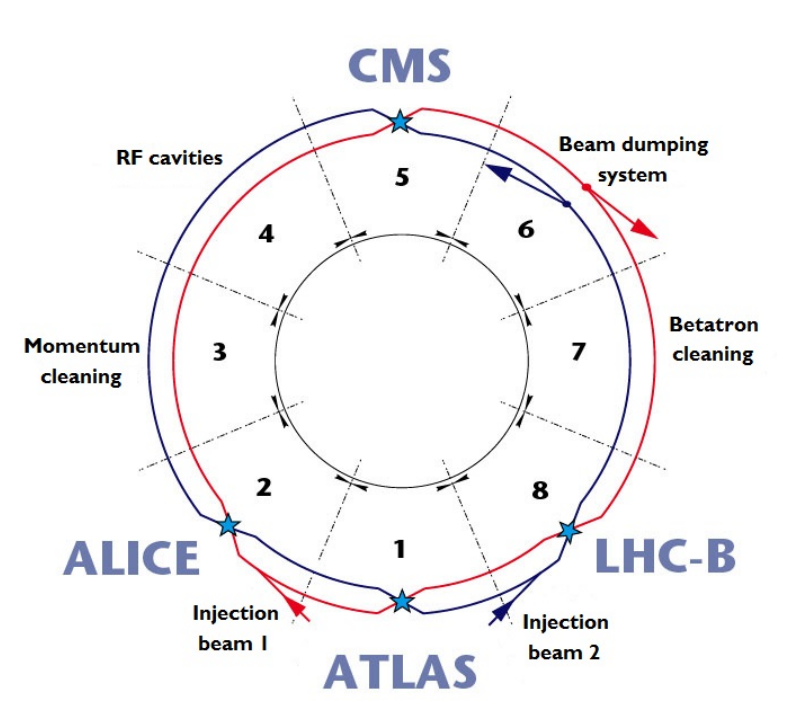
\includegraphics[width = 0.8\linewidth]{LHC_layout.png}
    \caption{Schematic overview of the LHC. The two beams circulate in opposite directions. Beam 1 (blue) is moving clockwise around the ring and beam 2 (red) moves counter-clockwise. The two beams can collide only in the regions containing the four experiments \cite{NorderhaugDrosdal:2015gkl}.}
    \label{fig:LHC_layout}
\end{figure}
\noindent The LHC layout follows the LEP tunnel geometry. The accelerator is divided into 8 sectors as shown in Figure \ref{fig:LHC_layout}. One sector extends from one straight section to the next containing one arc in between. The straight sections are named point 1 to point 8. The arcs are filled with the dipole bending magnets in a regular FODO\footnote{A FODO cell consists of a focusing quadrupole (FQ), a drift octapole (O), a defocusing quadrupole (DQ) and a second drift \cite{FODO}.} structure \cite{NorderhaugDrosdal:2015gkl}. The experimental regions with the detectors and other key equipment are placed in the straight sections. Currently, only 4 of these sections are occupied by detectors, where the beams intersect and share a common beam pipe for a short distance, forming the experimental insertions. The two general purpose detectors, ATLAS \cite{ATLAS:2008xda} and CMS \cite{CMS:2008xjf}, are located at diametrically opposed straight sections at interaction points 1 and 5 respectively. The two smaller experiments, ALICE \cite{ALICE:2008ngc} and LHCb \cite{LHCb:2008vvz} are located at point 2 and point 8, together with LHC’s beam injection points. The injection kick occurs in the vertical plane to the beams and the injection beams arrive at the LHC from below the reference plane. Points 3 and 7 contain two collimation systems each and point 4 contains RF systems that accelerate the beam particles. The beams are extracted from the machine at point 6 which contains the beam dump insertion. \\
\begin{figure}[H]
    \centering
    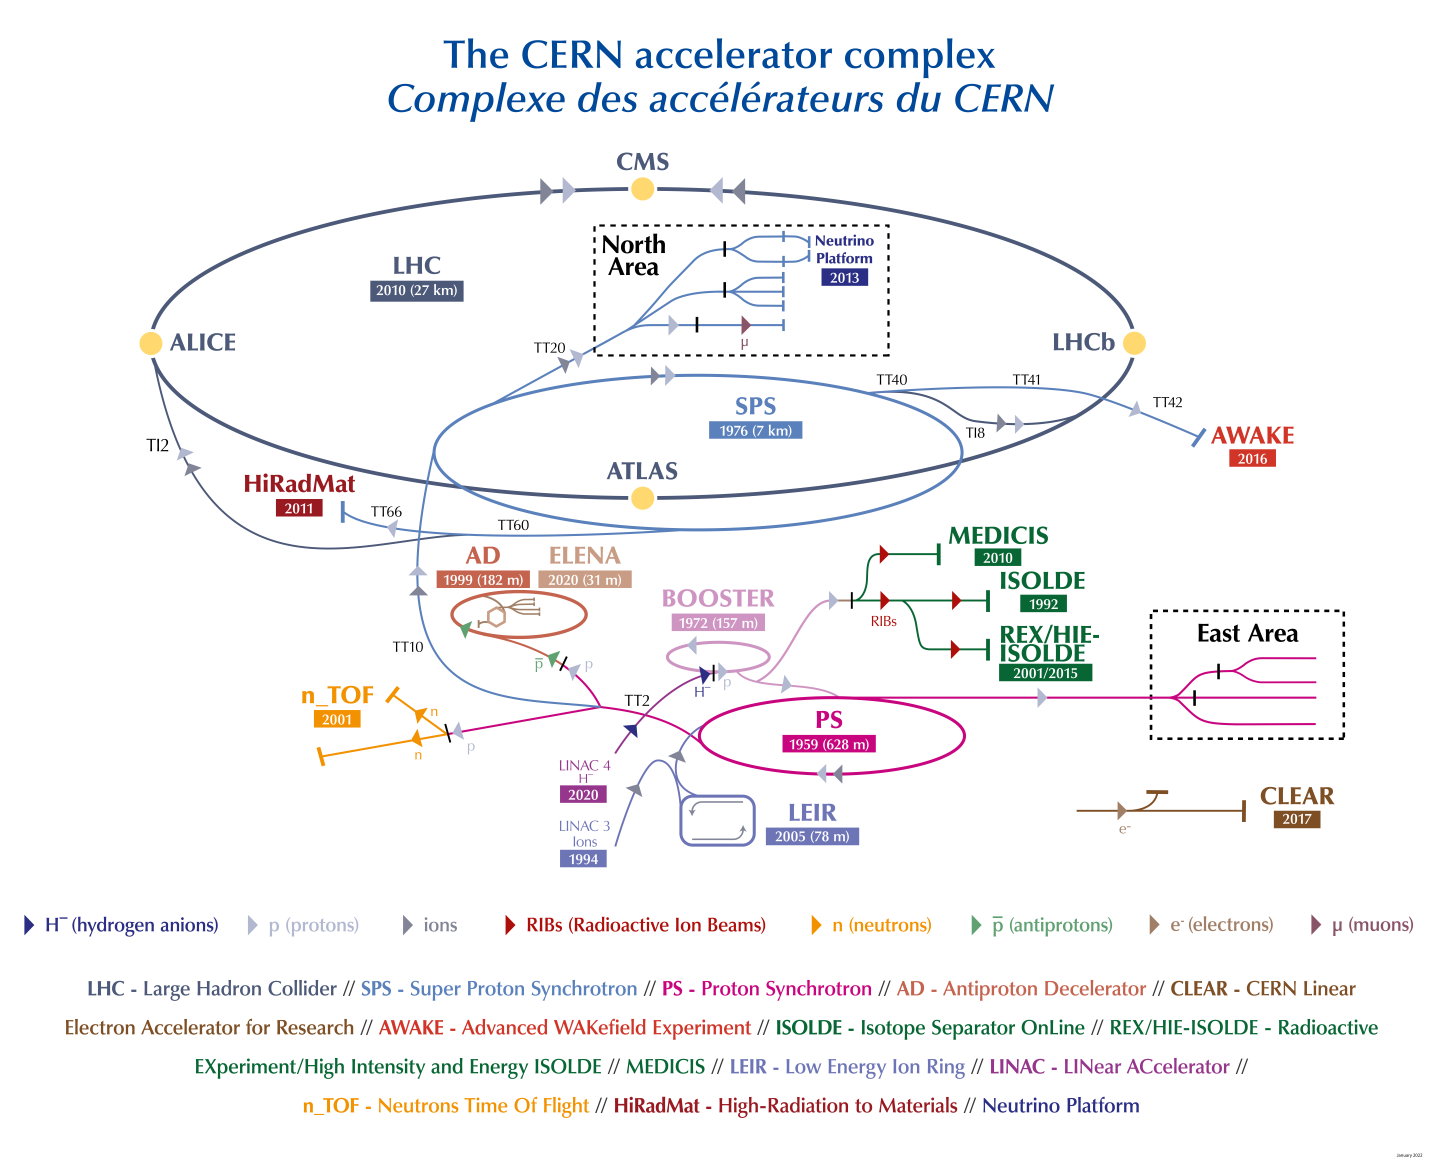
\includegraphics[width=0.9\linewidth]{LHC.png}
    \caption{The CERN accelerator complex \cite{Lopienska:2800984}}
    \label{fig:CERN accelarators}
\end{figure}
\indent As far as the acceleration of the beams, an accelerator complex consisting of multiple pre-acceleration steps is used, the last one being the LHC. The full accelerator complex at CERN is shown in Figure \ref{fig:CERN accelarators}. The source of the proton beam is a bottle of hydrogen gas. An electric field is used to strip hydrogen atoms of their electrons and yield protons. The first accelerator in the chain is LINAC 4\footnote{Before being replaced by LINAC 4 in 2020, the first accelerator was LINAC 2, which accelerated protons up to 50 MeV \cite{linac}} and accelerates the protons to energy of 160 MeV. Then the proton beam is injected into the Proton Synchrotron Booster (PSB) \cite{Schindl:1997cf} which accelerates protons to 1.4 GeV. The next in the accelerator chain is the Proton Synchrotron (PS) \cite{Cappi:1997vq} which pushes the proton beam up to 25 GeV and the Super Proton Synchrotron (SPS) \cite{Linnecar:1997wj} where the beam is further accelerated up to 450 GeV. Then the protons are split and injected in the LHC beam pipes where they circulate for about 20 minutes before they reach their final energy. Protons are aggregated in bunches containing $1.15 \cdot 10^{11}$ protons each. The bunches are separated in intervals of 25 ns.\\

\indent In the case of heavy ion operations, the LHC is filled with two beams of lead ions which pass through a similar acceleration chain as the protons. The lead ions are produced with an electron cyclotron resonance \cite{doi:10.1142/9789814436403_0023}. A very high plasma density can be attained by the use of microwave frequencies, thus adequate for the production of multi-charged ions. Many different charge states are obtained with a maximum around the charge state \ce{Pb^29+}. These are selected and accelerated to 4.2 MeV/u before passing through a carbon foil which strips further electrons off the lead ions yielding mainly \ce{Pb^54+}. The beam is then accumulated and accelerated to 72 MeV/u in the Low Energy Ion Ring (LEIR) \cite{Chanel:557588} and transferred to the PS, where it is further accelerated to 5.9 GeV/u. After passing the beam through a second foil where it is fully stripped to \ce{Pb^84+}, it is sent to the SPS for a last pre-acceleration to 177 GeV/u. This beam is then transferred to the LHC that accomplishes the final acceleration step before the beams are brought to collision. Table \ref{tab:LHC_accelerators} summarizes the pre-acceleration steps for both protons and lead ions and gives some of the design parameters of the LHC.

\begin{table}[H]
\centering
\caption{Overview of the accelerator complex for protons and lead ions. The different
accelerators, their design beam energy, and the ionization degree of the lead ions in each
phase are summarized in the upper part of the table. The lower part gives some design
parameters of the LHC machine.}
\label{tab:LHC_accelerators}
\begin{tabular}{cc||ccc}
\multicolumn{2}{c||}{Protons}                               & \multicolumn{3}{c}{Lead Ions}                             \\
Accelerator                     & Energy                   & Accelerator    & Energy        & \ce{^{208}Pb}  charge state  \\ \hline
LINAC 4                         & 160 MeV                   & LINAC 3        & 4.2 MeV/u     & \ce{Pb^29+}               \\
PSB                      & 1.4 GeV                  & LEIR           & 72 MeV/u      & \ce{Pb^54+}               \\
PS                              & 25 GeV                   & PS             & 5.9 GeV/u     & \ce{Pb^54+}                \\
SPS                             & 450 GeV                  & SPS            & 177 GeV/u     & \ce{Pb^84+}                \\
LHC                             & 7 TeV                    & LHC            & 2.76 TeV/u    & \ce{Pb^84+}                \\ \hline
\multicolumn{2}{c||}{2808 bunches}                          & \multicolumn{3}{c}{592 bunches}                           \\
\multicolumn{2}{c||}{$1.15 \cdot 10^{11}$ protons/bunch}     & \multicolumn{3}{c}{$7 \cdot 10^{7}$ lead ions/bunch}      \\
\multicolumn{2}{c||}{$\mathcal{L} = 10^{34} cm^{-2}s^{-1}$} & \multicolumn{3}{c}{$\mathcal{L} = 10^{27} cm^{-2}s^{-1}$}
\end{tabular}
\end{table}

\subsection{\label{sec:exp_LHC_2}Luminosity}
\noindent The luminosity $\mathcal{L}$ is one of the most important parameters of an accelerator. It is a measure of the flux density of beam particles created by the accelerator at the collision point. The number of collisions in a given time interval is given by 
\begin{equation}
    \frac{dN}{dt} = \mathcal{L} \sigma \Longrightarrow N = \sigma \int dt \cdot  \mathcal{L} 
\end{equation}
where $\sigma$ is the cross-section of the considered process. The machine's instantaneous luminosity depends only on the beam parameters and can be written as:
\begin{equation}
    \mathcal{L} = \frac{N_b^2 n_b f_{rev} \gamma_r}{4 \pi \epsilon_n \beta^{*}} F
\end{equation}
where $N_b$ is the number  of particles per bunch, $n_b $ the number of bunches per beam, $f_{rev}$ the revolution frequency, $\gamma_r$
the relativistic gamma factor, $\epsilon_n$ the normalized transverse beam emittance, $\beta^{*}$ the beta function at the collision point and F the geometric luminosity reduction factor due to the crossing angle at the interaction point:
\begin{equation}
    F = 1/ \sqrt{1 + \bigg(\frac{\theta_c \sigma_z}{2\sigma^{*}}\bigg)^2}
\end{equation}
where $\theta_c$ is the full crossing angle at the interaction point, $\sigma_z$ the RMS bunch length and $\sigma^{*}$ the transverse RMS beam size at the interaction point.
The design luminosity of the LHC is $\mathcal{L}= 10^{34} cm^{-2}s^{-1}$ for pp-collisions and $\mathcal{L} = 10^{27} cm^{-2}s^{-1}$ for the lead ion beams \cite{Brüning:782076}.

The integral of instantaneous luminosity over time is called integrated luminosity and it is a measure of the collected data size.
\begin{equation}
    L_{int} = \int dt \cdot \mathcal{L}
\end{equation}
Integrated luminosity is an important parameter that directly relates to the number of observed events. It is usually expressed in units of inverse femtobarn $ 1 \: \text{fb}^{-1} = 10^{39} cm^{-2} $. Figure \ref{fig:Lumi} shows the integrated luminosity delivered by the LHC and collected by the CMS experiment, during the Run 1 (2010-2012), the Run 2 (2015-2018) and Run 3 (2022-2023) data-taking for pp collisions.
\begin{figure}[htb!]
    \centering
    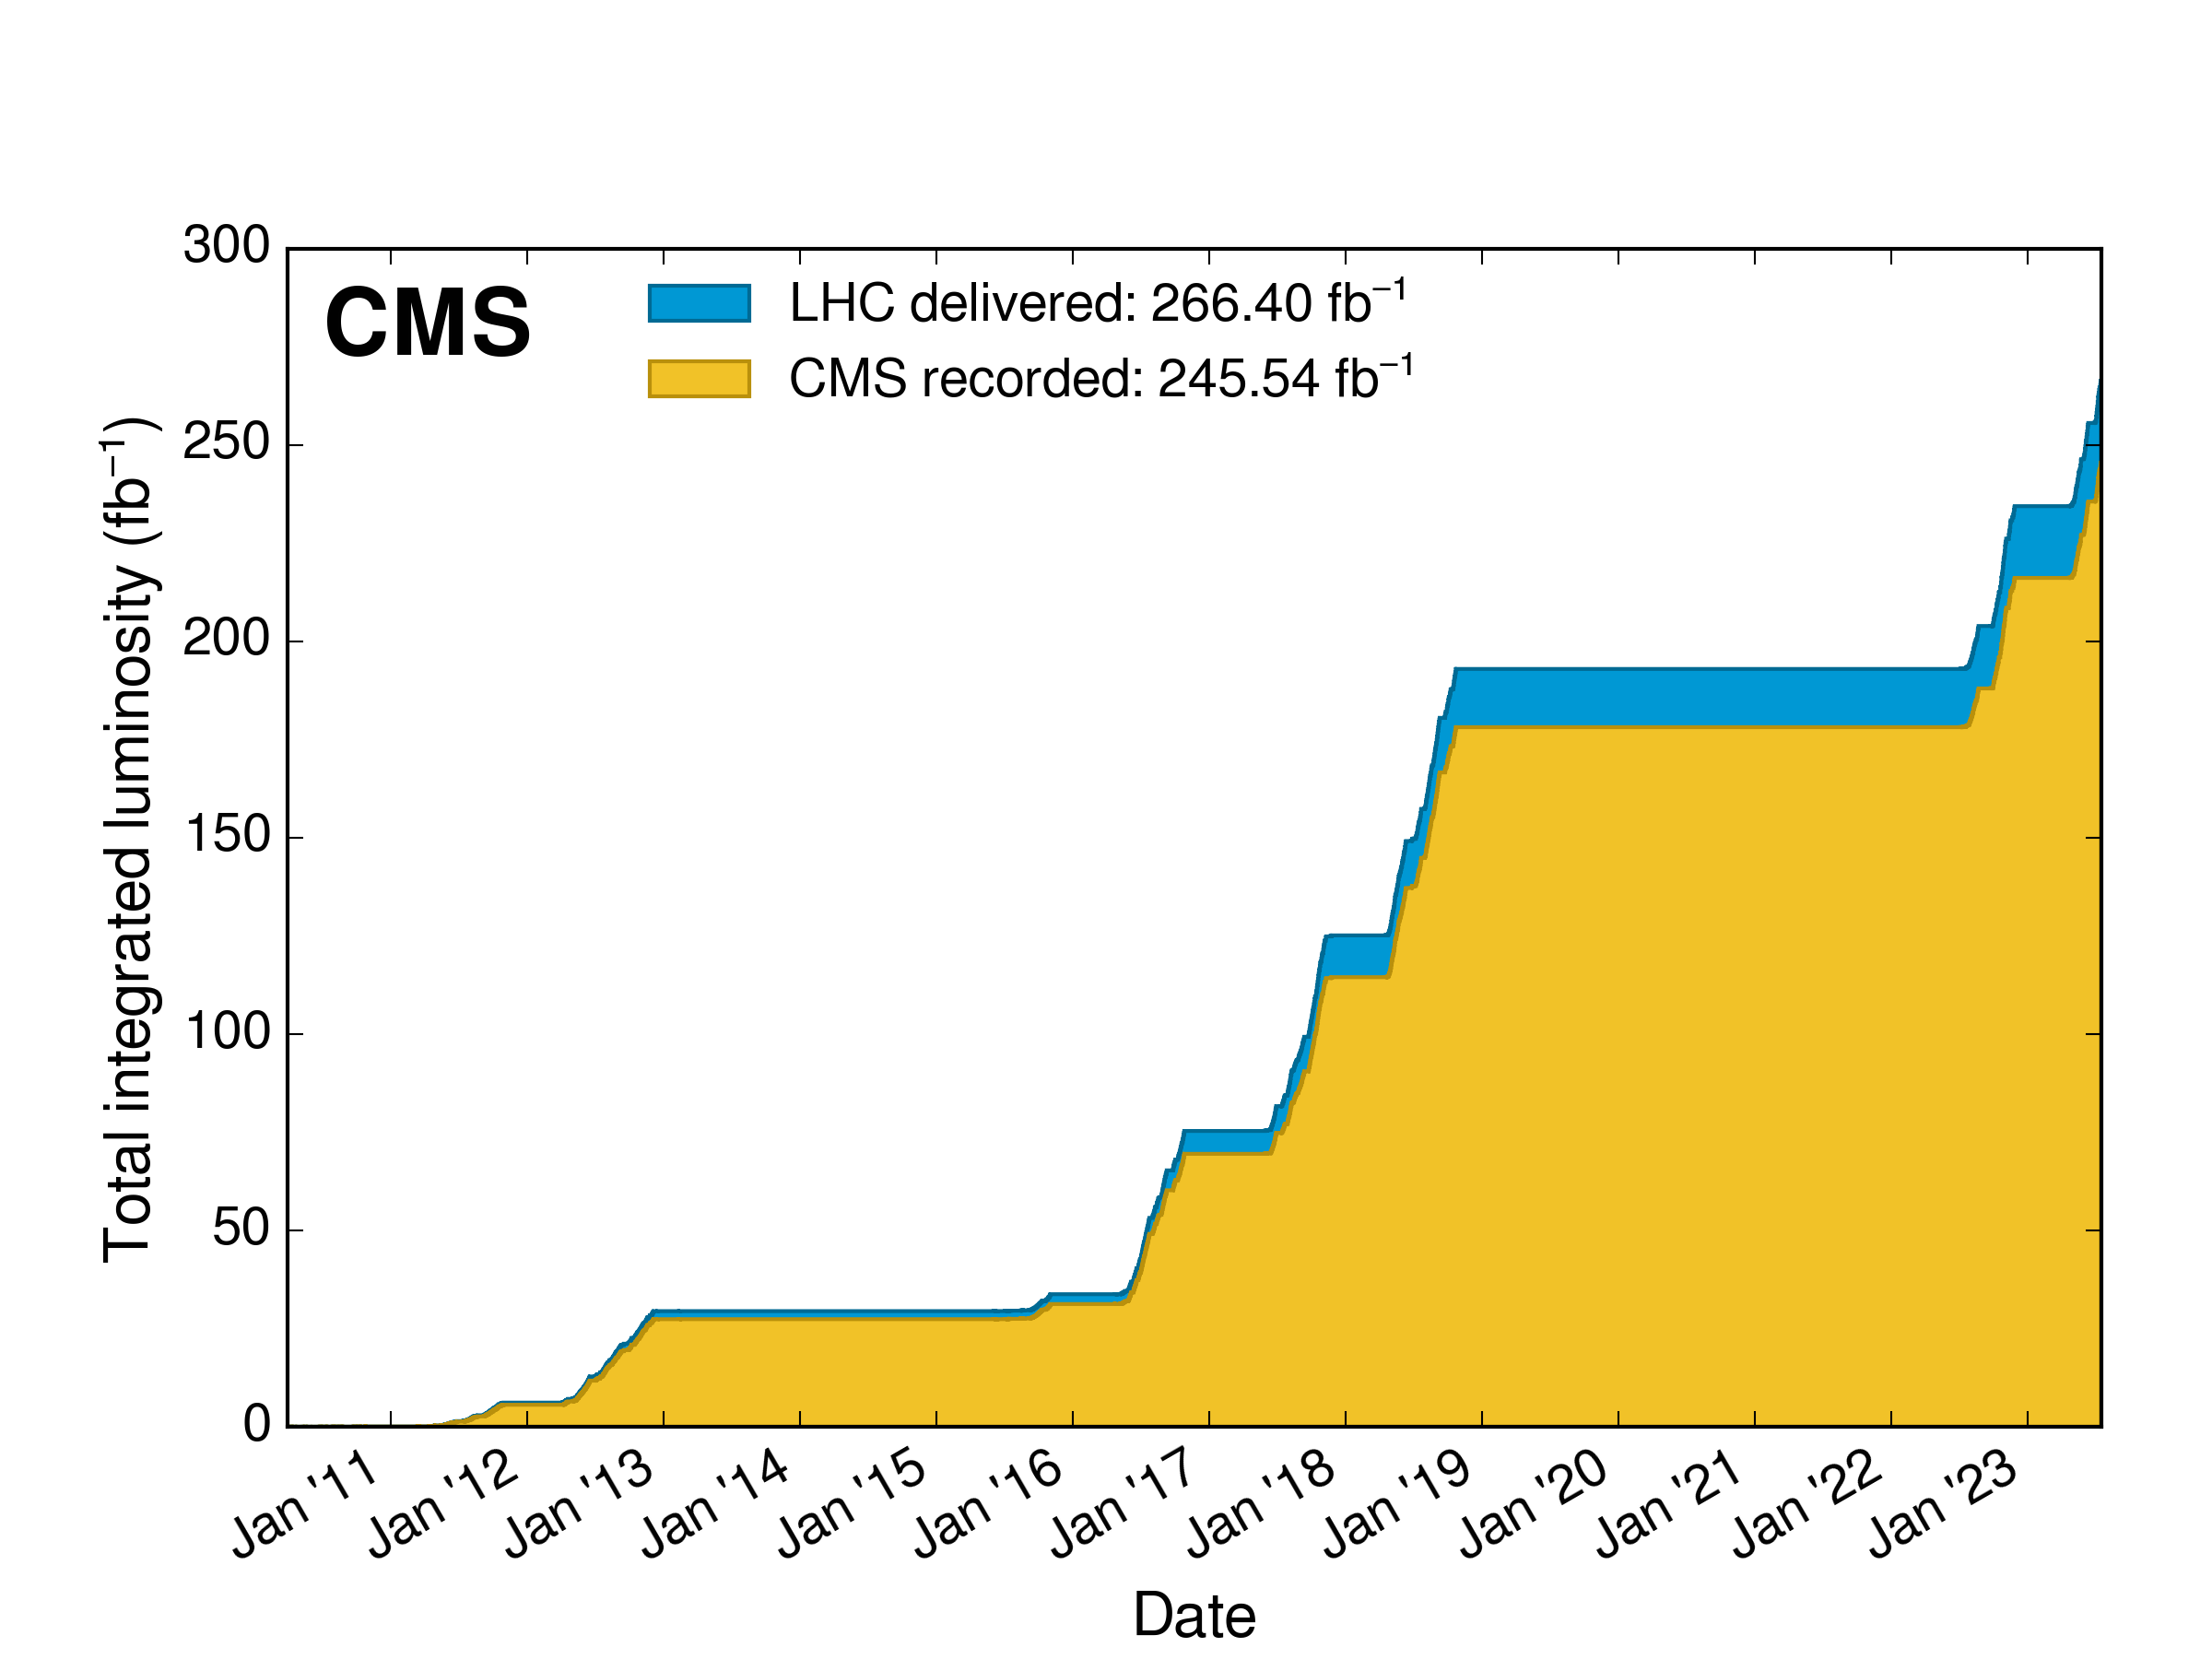
\includegraphics[width=0.65\linewidth]{Integrated_luminosity.png}
    \caption{Cumulative delivered and recorded luminosity versus time for 2010-2012, 2015-2018, and 2022-2023 (pp data only) \cite{IntLum}}
    \label{fig:Lumi}
\end{figure}
% The Run 1 of data taking lasted from 2010 to 2012. For the first year of this run LHC operated at a center-of-mass energy of $\sqrt{s}$ = 7 TeV and CMS collected integrated luminosity of $\sim 5.59 f b^{−1}$ . For the second part of Run 1, the center-of-mass energy was increased by 1 TeV and the experiment collected integrated luminosity of $ \sim 21.79 fb^{−1}$ . The LHC machine and the detectors were repaired and upgraded during a Long Shutdown (LS) 1 between 2013 and 2015. The data taking period from 2015 to 2018 is called Run 2. During that period LHC operated at 13 TeV and the integrated luminosity collected by CMS is $\sim 150.76 fb^{−1}$ . Currently, after another LS, the LHC machine undergoes its Run 3 which will last until 2025. After Run 3 a LS3 is programmed during which the machine will undergo major upgrades in order to prepare for HL-LHC.
The Run 1 of data taking lasted from 2010 to 2012. In its initial year, the LHC operated at a center-of-mass energy of $\sqrt{s}$ = 7 TeV, yielding an integrated luminosity of approximately $5.59 \: \text{fb}^{-1}$ collected by the CMS experiment. Subsequently, during the latter portion of Run 1, the  center-of-mass energy was elevated by 1 TeV, resulting in an integrated luminosity of around $21.79 \: \text{fb}^{-1}$. Following this phase, both the LHC apparatus and the detectors underwent maintenance and enhancements during a period known as Long Shutdown (LS) 1, spanning from 2013 to 2015. The subsequent data collection phase, termed Run 2, transpired from 2015 to 2018. Throughout this interval, the LHC operated at a  center-of-mass energy of $\sqrt{s}$ = 13 TeV, facilitating the accumulation of an integrated luminosity of approximately $150 \: \: \text{fb}^{-1}$ by the CMS experiment, of which approximately $140 \: \text{fb}^{-1}$ was certified as good for physics analysis. Presently and after another LS, the LHC is undergoing Run 3, slated to continue until 2025. For Run 3, the center-of-mass energy has once again increased to $\sqrt{s}$ = 13.6 TeV. Following the conclusion of Run 3, an LS3 is scheduled, during which the LHC will undergo significant upgrades in preparation for the High Luminosity LHC (HL-LHC).
%DATA QUALITY : https://twiki.cern.ch/twiki/bin/view/CMSPublic/DataQuality#Run_2_Data_Quality_Information


%\subsection{\label{sec:exp_LHC_3}High Luminosity LHC}

\section{\label{sec:exp_CMS}Compact Muon Solenoid Detector}
\noindent The Compact Muon Solenoid (CMS) detector is one of two largest general-purpose devices at the LHC and operates at interaction point 5. It has a length of 28.7 m, diameter of 15 m and it weights 14 ktonnes. It is designed to record all (stable) particles produced in the pp collisions, except of neutrinos (see Fig. \ref{fig:CMS}). As most particles produced in the pp collisions have lifetimes that are too short to be directly recorded in such a detector, mostly only the particles from the decay of primary particles are recorded in the detector itself. The origin of these particles, i.e. the process in the pp collision, has to be inferred via reconstruction algorithms and data analysis.\\
\indent CMS was initially conceived to unravel the mysteries surrounding electroweak symmetry breaking, particularly through the pursuit of the Higgs boson and searches for Beyond the Standard Model (BSM) phenomena at TeV energy scales such as natural supersymmetry. Now CMS has extended its physics program beyond these realms. A plethora of analyses are performed, exploiting the full range of pp and heavy-ion collision data.
\begin{figure}[H]
  \centering
  \begin{subfigure}{0.76\textwidth}
    \centering
    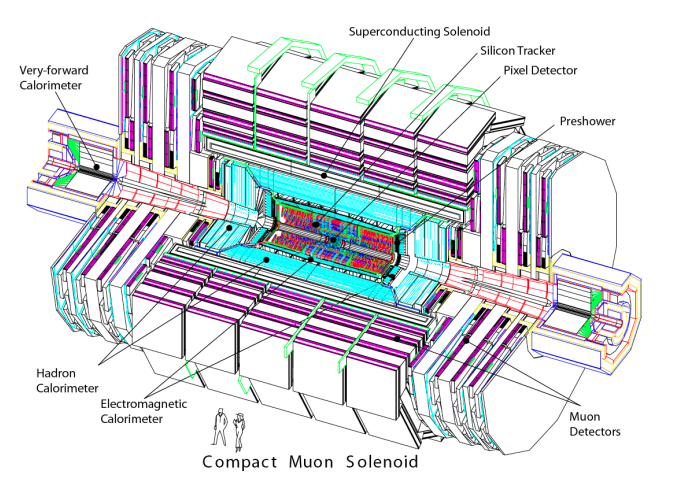
\includegraphics[width=1.0\linewidth]{CMS.png}
     \caption{}
    \label{fig:CMS}
  \end{subfigure}
  \hfill
  \begin{subfigure}{0.23\textwidth}
    \centering
    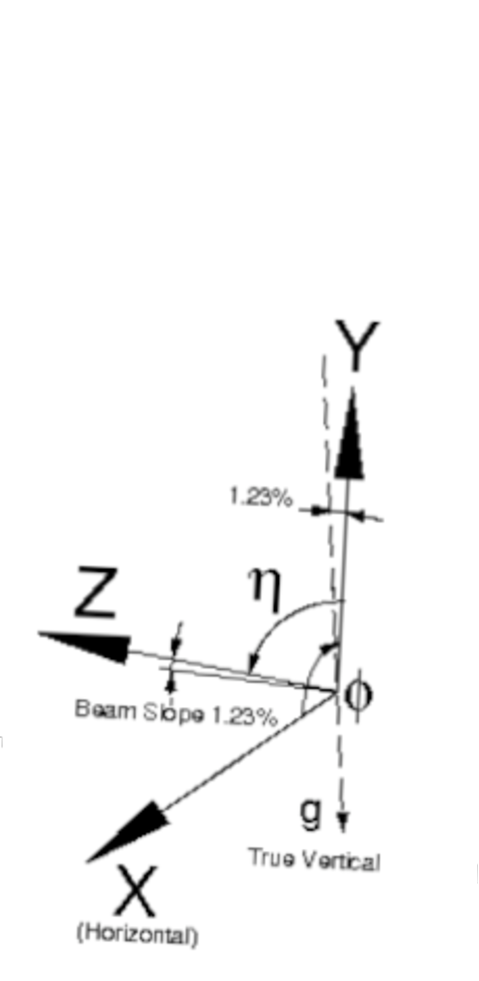
\includegraphics[width=1.0\linewidth]{CMS_cords.pdf}
     \caption{}
    \label{fig:CMS_Cords}
  \end{subfigure}
  \caption{(a) Schematic overview of the CMS detector \cite{CMS_sketch} and (b) the right-handed coordinate system \cite{CMS_cords}}
  \label{fig:CMS and cords}
\end{figure}

\subsection{\label{sec:exp_CMS_cords}Coordinate system and collider quantities}
\noindent At the CMS experiment, a right-handed coordinate system is used (Figure \ref{fig:CMS_Cords}), where the $x$ axis is defined towards the center of the LHC and the $y$ axis points upwards. The $z$ axis is defined in the direction of the beam. Since the plane of the LHC ring has a slight slope of 1.23\% with respect to the horizontal by construction, the coordinate system of CMS is tilted accordingly. The CMS detector is cylindrical with the center being the pp interaction point. Correspondingly, an azimuthal angle $\phi$ is defined in the ($x$, $y$)-plane, and a polar angle $\theta$ relative to the beam direction. The collisions and resulting processes are symmetrical in $\phi$.\\
\indent Both colliding beams feature protons with identical energies, resulting in equal but opposite momenta along the $z$ direction, while exhibiting negligible momentum in the ($x$,$y$)-plane. Since protons are composite particles, their constituent partons are the entities that undergo collisions, behaving as quasi-free particles due to the asymptotic freedom of QCD. The momentum fraction carried by the partons in a single proton-proton collision remains uncertain, rendering the total momentum along the $z$ direction indeterminate. Consequently, it is convenient to define a quantity that is invariant against (unknown) boosts in the $z$ direction, such as the transverse momentum.
\begin{equation}
    p_T = \sqrt{p_x^2 +p_y^2}
\end{equation}
The transverse momentum quantifies the momentum in the ($x$,$y$)-plane.\\
\indent Another common quantity is the rapidity, $y$, which is defined as
\begin{equation}
    y = \frac{1}{2} \bigg( \frac{E+p_z}{E-p_z}\bigg)
\end{equation}
Differences in the rapidity are invariant against Lorentz boosts along the $z$ direction, resulting in a suitable quantity to measure the angular separation of two particles. \\
\indent However, because of the high energies that we encounter  in particle physics, we are interested in the limit where  $|\vec{p}|  \gg m$, i.e. the limit where $m \rightarrow 0$. In this limit the rapidity takes another form, which we call pseudorapidity, $\eta$:
\begin{equation}
    \eta \equiv \lim_{m \rightarrow 0} \frac{1}{2} \ln\bigg( \frac{E+p_z}{E-p_z}\bigg)
\end{equation}
which, because $E \approx |\vec{p}|$ and $p_z = |\vec{p}| \cos\theta$, can be written as:
\begin{equation}
    \eta = \frac{1}{2} \ln\bigg( \frac{ |\vec{p}| +|\vec{p}|\cos\theta}{|\vec{p}|- |\vec{p}| \cos\theta}\bigg) = \frac{1}{2} \ln\bigg( \frac{ 1 +\cos\theta}{1 - \cos\theta}\bigg) = -\ln\bigg[ \tan\bigg( \frac{\theta}{2} \bigg) \bigg]
\end{equation}
The pseudorapidity is defined such that $\eta = 0$  is perpendicular to the beam axis and $\eta \rightarrow \pm \infty$ is parallel to the beam axis (Figure \ref{fig:pseudorapidity}). Angular distances in the ($\theta$, $\phi$)-plane are usually quantified with $\Delta$R,
 \begin{equation}
     \Delta R= \sqrt{(\Delta\phi)^2 + (\Delta\eta)^2}
 \end{equation}
using the pseudorapidity $\eta$ instead of the polar angle $\theta$
\begin{figure}[H]
    \centering
    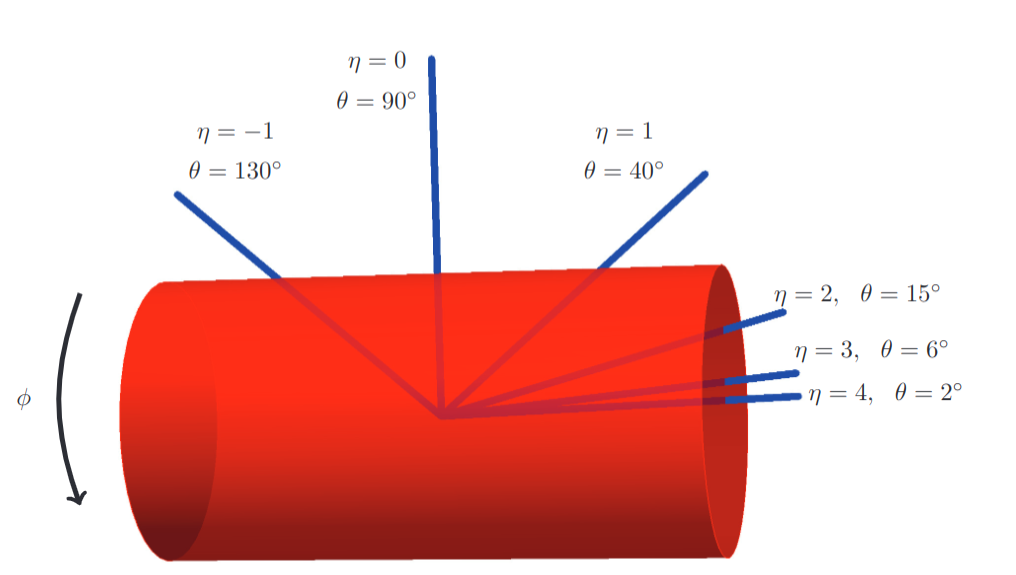
\includegraphics[width=0.5\linewidth]{pseudorapidity.png}
    \caption{Pseudorapidity as a function of the polar angle $\theta$ \cite{Schwartz_2018}}
    \label{fig:pseudorapidity}
\end{figure}

\subsection{\label{sec:exp_CMS_layout}CMS layout}
\noindent The detector's geometry is specifically designed for optimal particle detection and maximum reconstruction performance. It is cylindrical, with its axis along the beam line and the collision region centered at its geometrical center. Comprising the central region are the barrel sections, constructed from 5 distinct wheels, while the forward regions are covered by disks known as endcaps. The structure of the detector resembles that of a cylindrical onion, i.e. it consists of several concentric layers, each of which is designed for a different purpose. The interaction of the colliding particles with the detector materials result in electric signal. This signal is measured, digitised and finally analysed by computers.

\begin{figure}[H]
    \centering
    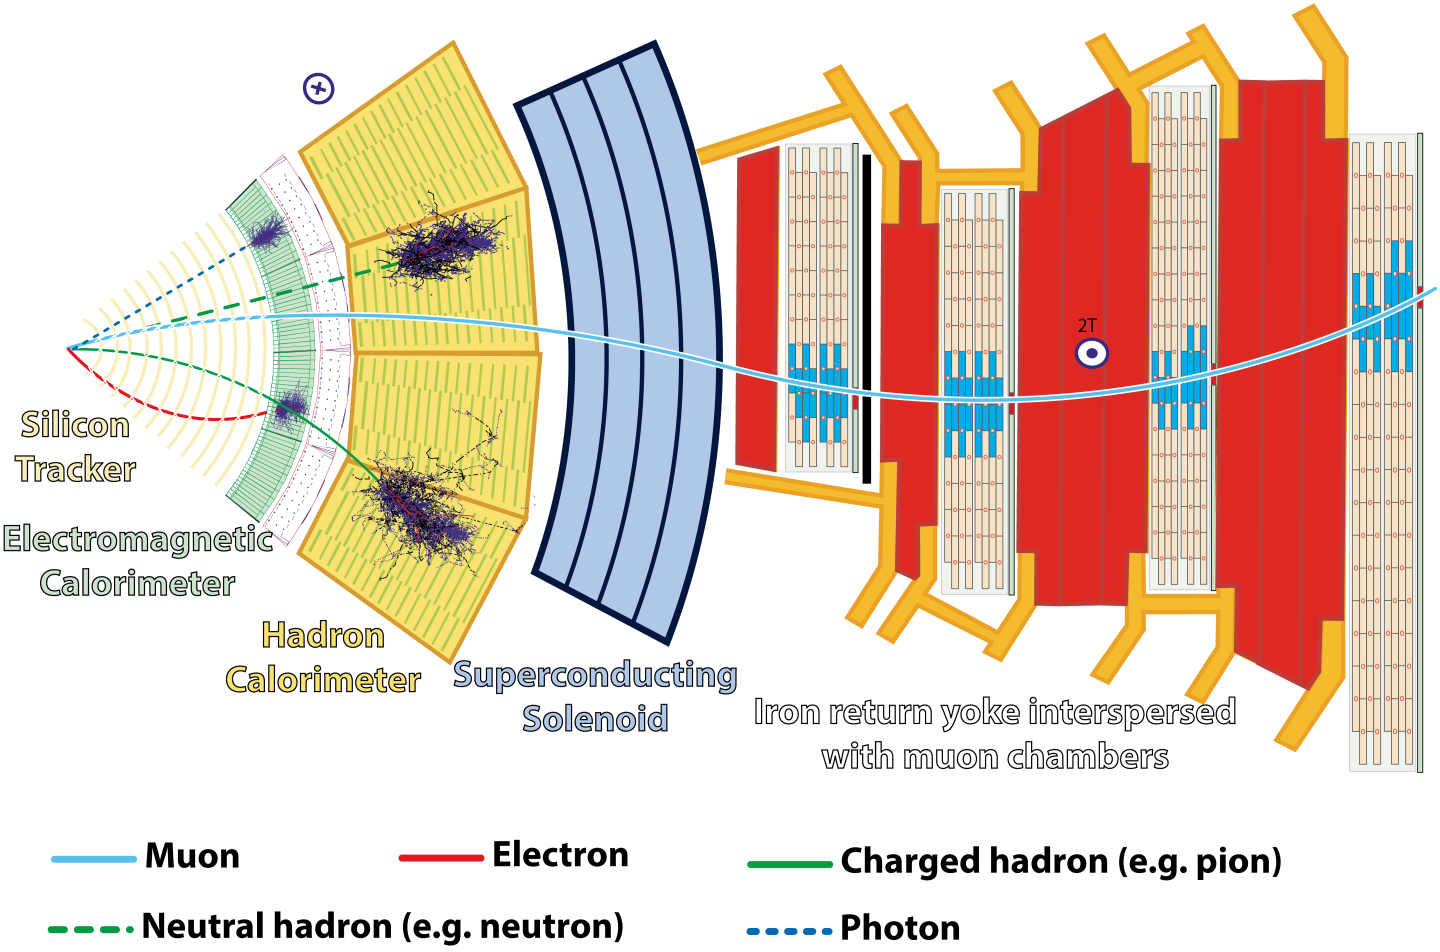
\includegraphics[width=0.7\linewidth]{CMS_layout.png}
    \caption{Slice showing CMS sub-detectors and how particles interact with them \cite{CMS_slice}}
    \label{fig:CMS_slice}
\end{figure}

As shown in Figure \ref{fig:CMS_slice}, the barrel is comprised of five main parts. The tracker is a cylinder of 5.8 m long and diameter of 2.6 m. Its purpose is the identification of charged particles and the measurement of their trajectories, momenta and charges. Outside the tracker, the electromagnetic and hadronic calorimeters are located sequentially. The electromagnetic calorimeter (ECAL) is designed to detect electrons and photons and surrounds the tracker with an outer radius of 1.75 m. The hadronic calorimeter (HCAL) is designed to detect jets of hadrons and has an outer radius of 3 m.\\
%The electromagnetic calorimeter (ECAL), which is a cylinder with diameter of 3.5 m and lenght of 7.8 m, is designed to detect electrons and photons, while the hadronic calorimeter (HCAL) is designed to detect jets of hadrons.\\
\indent The precise momentum measurement of high-energy charged particles requires large bending power by a strong magnetic field. This is achieved by the main feature of the CMS detector, the superconducting solenoid magnet. It generates a 3.8 T, nearly homogeneous magnetic field, parallel to the beam line. The large magnetic field provides strong bending on the muon tracks, before they enter the muon chambers. The solenoid accommodates the tracker and the calorimeters within its volume.\\
\indent Outside the solenoid, the muon system is integrated in the iron return yoke frame which confines the magnetic field outside the solenoid to allow for momentum measurement with the muon detectors, as well as to protect the detector electronics. The muon detection utilizes gas ionization technology and its purpose is to identify and measure the momentum and charge of the muons.\\
\indent The detector has almost full solid angle coverage. The central barrel region covers up to $|\eta| < 1.48$ and the two endcaps cover up to $|\eta| < 3$. In the very forward regions of HCAL the coverage of pseudorapidity is extended to $\eta = 5$.\\
\indent The following subsections describe the different detector components, starting at the nominal interaction point in the center of the detector and following the geometric order radially outwards. A detailed review of the CMS detector can be found in \cite{CMS:2008xjf, CMS_sketch}

\subsection{\label{sec:exp_CMS_1}Inner tracking system}
\noindent The innermost part of the CMS detector is the tracking system. Its purpose is to provide precise and efficient measurement of charged particle trajectories through the ionization they produce along their path. Charged particles traversing the tracker induce electron-hole pairs, which create measurable currents that are digitized. The resulted “hits” are grouped into tracks using advanced pattern recognition algorithms and reconstruct a trajectory per particle. The origin or "vertex" and the direction of flight of the particle are also indicated by the reconstructed trajectory.
\begin{figure}[H]
    \centering
    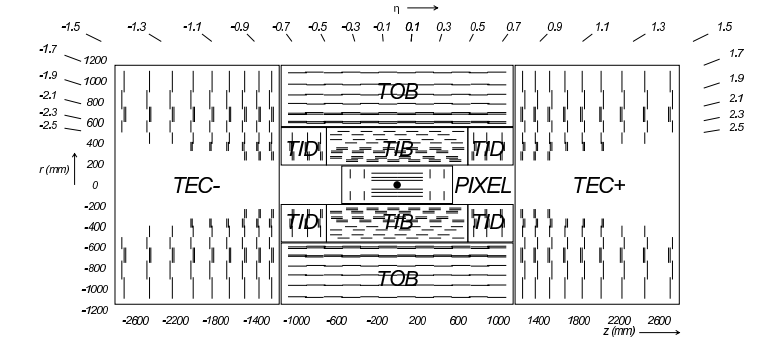
\includegraphics[width=0.8\linewidth]{Tracking_system.png}
    \caption{Schematic overview of the CMS tracking system \cite{CMS:2008xjf}. The silicon pixel detector in the center is surrounded by the silicon strip detector which consists of endcaps and different barrel components.}
    \label{fig:Tracking_system}
\end{figure}
\indent The tracker is required to have high granularity, fast response and high radiation and age resistance. Therefore, silicon technology was used for the construction of the tracker. The tracker was designed to operate without loss of efficiency up to an integrated luminosity of $500 \: \text{fb}^{-1}$. The solenoid magnet covers fully the tracker, whose total sensitivity area is $200 m^2$ and its acceptance expands up to $|\eta| < 2.5$. \\
\indent The tracker consists of five parts as depicted by Figure \ref{fig:Tracking_system}:
\begin{enumerate}
    \item Pixel Detector: 4 concentric barrel layers of $285 \: \mu m$ thick sensors at $r = 2.9, 6.8, 10.9$ and $16.0\: \text{cm}$, covering up to $|z| < 27 \: \text{cm}$  and three disks, $300 \mu m$ thick each at distances of $|z|$ = 29.1, 39.6, and 51.6 cm.
    \item Tracker Inner Barrel (TIB): 4 barrel layers of $320\: \mu m$ thick sensors, covering up to $|z| < 65 \: \text{cm}$ and $20 < r < 55\: \text{cm}$, configured parallel to the beam line.
    \item Tracker Inner Disks (TID): 3 disks at each end covering $65< |z| < 120\: \text{cm}$ and $20 < r < 55\: \text{cm}$. Each micro-strip sensor is $320 \: \mu m$ thick, configured radially.
    \item Tracker Outer Barrel (TOB): 6 barrel layers of sensors, $500 \: \mu m$ thick. Extends in radius from $55 < r < 116\: \text{cm}$ and withing $|z|<118 \:\text{cm}$, surrounding the TIB/TID.
    \item Tracker End Caps (TEC): Each TEC is composed of 9 disks, $320-500 \:\mu m$ thick. They are configured in the radial direction, covering the region $124< |z| <282\: cm$ and $22.5<|r|< 116 \:cm$. 
\end{enumerate}
All parts apart from the Pixel Detector are made out of silicon microstrips. The tracker transverse momentum resolution for high momentum tracks (100 GeV) in the central region ($|\eta| < 1.6$) is 1-2\% and degrades at higher $\eta$. For lower momentum tracks the transverse momentum resolution of the tracker is dominated by multiple scattering. The transverse and longitudinal impact parameter resolution is 10 $\mu$m for high momentum tracks while it reduces at lower momentum due to multiple scattering.

\subsubsection{\label{subsubsec:exp_CMS_pixel} Silicon pixel detector}
\begin{figure}[H]
    \centering
    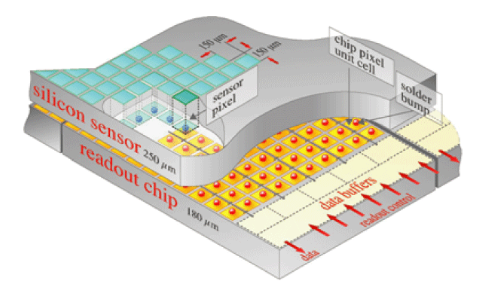
\includegraphics[width=0.5\linewidth]{Pixelement.png}
    \caption{Sketch of a typical pixel sensor used in the pixel detector \cite{Silicon_Pixels}}
    \label{fig:Silicon_pixel}
\end{figure}
\noindent The Pixel Detector contains 124 million pixels and allows the tracks reconstruction with extreme accuracy. After the end of 2016 data taking period the pixel detector was replaced with an upgraded version called CMS Phase-1 pixel detector \cite{Adam_2021, Dominguez:1481838}. The layout of the CMS Phase-1 pixel detector is optimized to have four-hit coverage over the pseudorapidity range $|\eta| < 2.5$, improved pattern recognition and track reconstruction, and added redundancy to cope with hit losses.\\
\indent Each of the four layers is composed of individual silicon modules, splitted into little silicon sensors, the pixels (Figure \ref{fig:Silicon_pixel}). Each of these silicon pixels is $100\: \mu m \times 150\: \mu m$, about two hairs widths. When a charged particle passes through a pixel, it gives enough energy to eject the electrons from silicon atoms, thus creating electron-hole pairs. A voltage applied to the sensor allows collecting these charges as a small electric signal, which is amplified by an electronic readout chip (for a total of 16 chips per module). Knowing which two-dimensional pixels and in which layer has been touched allows us to deduce the three-dimensional particle’s trajectory.
\subsubsection{\label{subsubsec:exp_CMS_strip} Silicon strip detector}
\noindent Covering an area of 223 $m^2$ with axial range of 20 to 116 cm, the tracker houses 10 million Strip Silicon Detectors. It contains 15,200 modules, read by 80,000 microelectronic chips, designed to withstand radiation at $-20^\circ$C. While pixels focus on recording precise three-dimensional particle trajectory data, strip trackers capture more rough two-dimensional information across multiple surfaces, enhancing momentum measurement accuracy. 
\begin{figure}[H]
    \centering
    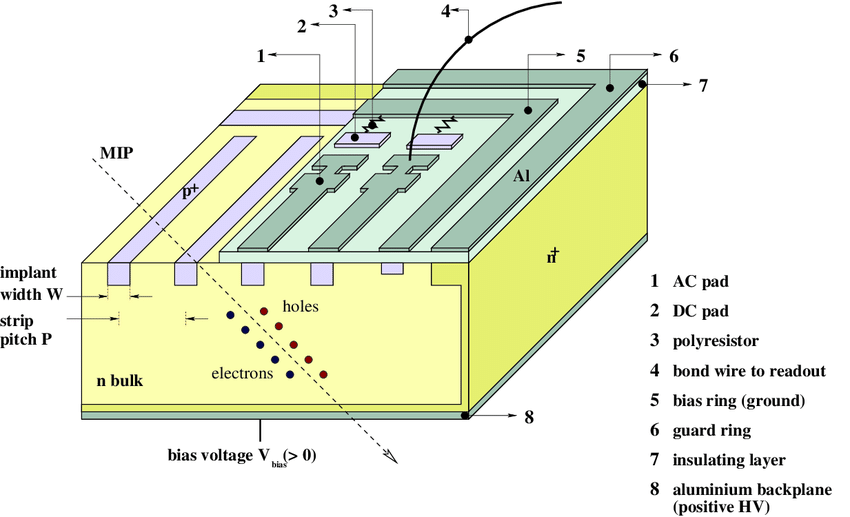
\includegraphics[width=0.5\linewidth]{Microstrip.png}
    \caption{Schematic structure of a CMS silicon microstrip sensor \cite{Axer:2003ata}.}
    \label{fig:Silicon_microstrip}
\end{figure}
As mentioned above, the strip tracker, is formed by four sub-modules forming a ten-layered silicon strip detector, extending to a radius of 116 cm. The silicon detectors work in much the same way as the pixels: as a charged particle crosses the material it knocks electrons from atoms giving a very small pulse of current lasting a few nanoseconds. Analogue Pipeline Voltage (APV25) chips amplify this small amount of charge, giving us “hits” when a particle passes, which allow for the reconstruction of its path \cite{Silicon_Strips}. Signals are processed, converted into infrared pulses, and transmitted for analysis via fiber optic links.


\subsection{\label{sec:exp_CMS_2}Electromagnetic Calorimeter}
The ECAL is almost a hermetic homogeneous\footnote{The entire volume is sensitive and contributes a signal} detector layer that surrounds the
tracker \cite{CMS_sketch, Chatrchyan:1215500, Collaboration_ECAL, ECAL, CERN:ECAL}. It is composed of 75848 lead tungstate ($\ce{PbWO4}$) crystals designed to measure the energy of the particles that interact primarily via the electromagnetic interaction, i.e. electrons and photons. Electrons emit numerous Bremsstrahlung photons due to electromagnetic interactions, while photons engage with matter via the photoelectric effect, Compton scattering, and pair production.
\begin{figure}[H]
    \centering
    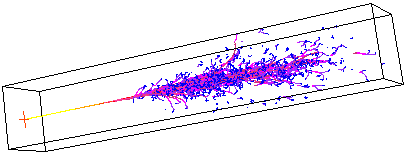
\includegraphics[width=0.5\linewidth]{Simulated_shower.png}
    \caption{Simulated cascades inside electromagnetic crystals \cite{Menke}.}
    \label{fig:Shower}
\end{figure}
When a particle arrives, it interacts, generating numerous softer particles with reduced energy levels successively. This cycle continues, resulting in the creation of multiple low-energy particles, forming what is known as a cascade shower. This progression halts when the generated particles lose adequate energy and are absorbed by the material they traverse. The Molière radius is a characteristic constant of a material giving the scale of the transverse dimension of the fully contained electromagnetic showers initiated by an incident high energy electron or photon. Molière radius, $R_M$, is given by \cite{Workman:2022ynf}
\begin{equation}
    R_M = X_0 \frac{E_s}{E_C}
\end{equation}
where $E_s$ = 21 MeV and $E_C$ is the critical energy at which the ionization and bremsstrahlung rates are equal. $X_0$\footnote{$X_0$ is usually measured in $g\cdot cm^{2}$}, is another characteristic constant of the materials, the radiation length. The radiation length, defines the average length an electron has to travel to reduce its initial energy by $1/e$ or the $7/9$ of the mean free path of a photon. The shower's depth depends on the initial particle's energy as:
\begin{equation}
    X = X_0\frac{ln\big(E_0/E_C\big)}{ln2}
\end{equation}
where $E_0$ is the initial particle energy. If the energy of the shower is smaller than the critical energy, the shower stops. Both the radiation length and the Molière radius depend on the detector’s material and need to be low enough in order to achieve compact calorimeters.\\
\indent Lead tungstate crystal is chosen to be the active material, i.e. where all the electromagnetic processes take place, since it satisfies all of the above prerequisites. It is highly dense ($8.28 g/cm^3$), it has a short radiation length ($X_0 = 0.89 cm$) and a small Molière radius ($R_M = 2.2 cm$). It is also very fast responding, about 80\% of the scintillation light in the crystals is emitted within 25 ns, the LHC bunch crossing time. The crystals are also radiation-hard, with the ability to maintain a good ECAL performance throughout LHC operations.
\begin{figure}[H]
    \centering
    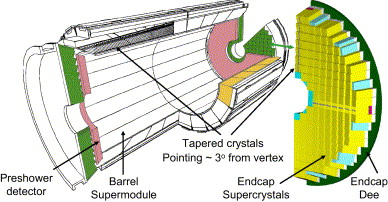
\includegraphics[width=0.7\linewidth]{ECAL.png}
    \caption{A schematic view of the CMS Electromagnetic calorimeters \cite{ECAL}.}
    \label{fig:ECAL}
\end{figure}
\indent As electrons and photons pass through the ECAL, their electromagnetic shower results in cascades giving rise to scintillation in the crystals. Avalanche photodiods (APDs) are used as photodetectors in the barrel and Vacuum phototriods are used in the endcaps (VPT). The lateral size of the crystals is $\sim 1R_M$ and hence 90\% of the EM shower can be contained within a single crystal. The number of scintillation photons that will be emitted by the crystals and the amplification of the photodetectors depend on the temperature. A cooling system is used to keep the temperature of the system constant.\\
\indent Figure \ref{fig:ECAL} shows the structure of ECAL. It consists of the barrel region, ECAL Barrel (EB), and the endcap region, ECAL Endcaps (EE). The EB is located at a radial distance between 129 and 175 cm, covers up to $|\eta| < 1.479$ and contains 61200 crystals. Each crystal has a length of $23 cm$ and a radiation length of $25.8 X_0$. The crystals are formed into 36 “supermodules”, each weighing around three tonnes and containing 1700 crystals. The EE are located $\pm 317 cm$ from the nominal collision point, covering an interval of $1.479 < |\eta| < 3.0$ and containing 7324 crystals, each 22 cm long. In front of these crystals, there is the ECAL Preshower (ES) detector, covering an area of $1.653 < |\eta| < 2.6$. It has a total width of 20 cm and consists of two lead plates and two silicon plates, arranged alternately. It is used to distinguish between photons and the neutral pions $\pi^0$. These short-lived particles are produced at a very high rate during proton collisions and decay mainly into two lower energy photons which are spatially close together. For this reason, the detection strips of the preshower detector have a width of only 2 mm, thus offering higher resolution and higher precision than other calorimeter systems, making it possible to distinguish the two photons from the decay of neutral pions.\\
\indent The energy resolution of the ECAL has been measured in test beams to be \cite{CMS:2008xjf}:
\begin{equation}\label{eq:ECAL}
    \bigg( \frac{\sigma}{E}\bigg)^2 = \bigg(\frac{2.8\%}{\sqrt{E}}\bigg)^2 + \bigg(\frac{12.0\%}{E}\bigg)^2 + (0.3\%)^2
\end{equation}
with E measured in GeV. The first term in Eq. \ref{eq:ECAL} is the stochastic term and parameterizes the intrinsic energy fluctuations of the shower. The second term is the noise term and accounts for electronic and digitization noise or energy fluctuations from external to the shower sources. The last term is the constant term and accounts for calibration errors or leakage of the EM shower. Since it is a homogeneous calorimeter, the effect of the very small stochastic and noise term become negligible at $50$ GeV. The real challenge for the ECAL energy resolution at high energy is the constant term \cite{Cavallari_2011}.
\subsection{\label{sec:exp_CMS_3}Hadronic Calorimeter}
The HCAL \cite{HCAL} is a sampling calorimeter\footnote{The material that produces the particle shower is distinct from the material that measures the deposited energy} that consists of alternating layers of brass or stainless steel as absorber and plastic scintillator or quartz fiber tiles as sensitive material that measures the energy deposit. Its main purpose is the absorption and energy measurement of strongly interacting particles. These particles create hadronic showers in the brass layer and induce detectable light in the scintillator which is guided by embedded wavelength-shifting fiber to readout electronics \cite{CERN:HCAL,Mans:1481837}.\\
\indent In contrast with the electromagnetic cascades, the physical processes leading to the formation of hadron showers are different. Hadron production, nuclear deexcitation and meson decays predominate in these showers. Approximately one-third of the produced pions are neutral whose energy is dissipated in the form of electromagnetic showers. It is very often that a hadronic shower has also an electromagnetic component which sometimes can be a bit displaced from the hadronic one because of the magnetic field.\\
\indent Additionally, hadronic showers differ in their development duration compared to electromagnetic ones. This can be seen by comparing the number of particles present versus depth for pion and electron initiated showers. The longitudinal development of hadronic showers scales with the interaction length. For this reason hadronic calorimeters are longer and bigger than the electromagnetic calorimeters, in order to include the whole cascade and avoid as much as possible energy and particles losses from the back parts of the alternating layers of active material and absorber plates.
\begin{figure}[H]
    \centering
    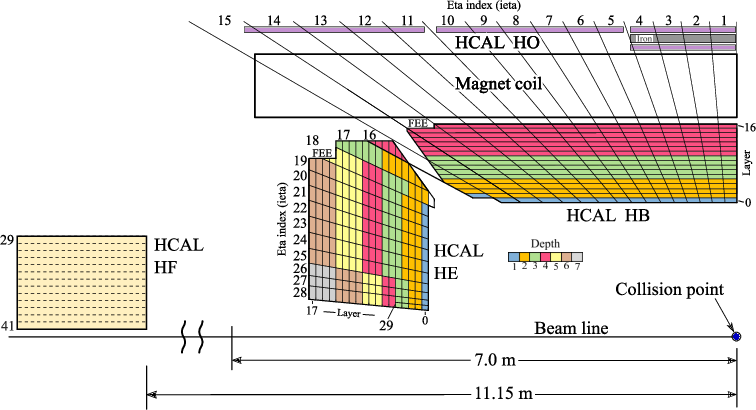
\includegraphics[width=0.9\linewidth]{HCAL2.png}
    \caption{A quadrant of the CMS hadronic calorimeter \cite{Hayrapetyan:2870088}.}
    \label{fig:HCAL}
\end{figure}
\indent The HCAL consists of four parts arranged in the layout shown in Figure \ref{fig:HCAL}. The Hadronic Barrel (HB) and the Hadronic Endcaps (HE) calorimeters surround the ECAL and are located inside the superconducting solenoid. The Hadronic Outer (HO) calorimeter is placed just outside the solenoid complementing the HB and the Hadronic Forward (HF) calorimeter is located $11.15$ m away from the interaction point. The angle coverage of HCAL reaches up to $|\eta| < 5.2$. \\
\indent The design of the HCAL was significantly influenced by the choice of magnetic parameters, since the detector array, with the exception of the HO section, is located within the solenoid magnet. Thus, brass was chosen for the absorber material as it has a relatively short interaction length and is non-magnetic, while plastic scintillator plates were used as the active material.\\
\indent The combined energy resolution of the CMS HCAL+ECAL for pions that was measured during a test-beam analysis is (after correction) \cite{Cavallari_2011}:
\begin{equation}\label{eq:HCAL}
    \bigg( \frac{\sigma}{E}\bigg)^2 = \bigg(\frac{84.7\%}{\sqrt{E}}\bigg)^2 + (7.4\%)^2
\end{equation}
The noise term is found to be negligible. Similar energy resolution was found also in the endcaps. Comparing the stochastic term of the Equation \ref{eq:HCAL} with the corresponding one from the ECAL (Eq. \ref{eq:ECAL}), we notice that this term, in the case of the HCAL, is bigger. This happens because the HCAL is a sampling calorimeter and not homogeneous. The HF energy resolution from test beam \cite{HCAL_2007} is:
\begin{equation}
     \bigg(\frac{\sigma}{E}  \bigg)^2 =  \bigg(\frac{280\%}{\sqrt{E}} \bigg)^2 + (11 \%)^2
\end{equation}
\subsection{\label{sec:exp_CMS_4}The magnet}
\noindent Immediately after the hadronic calorimeter we find the superconducting solenoid \cite{Solenoid_5,Solenoid_1, Solenoid_2, Solenoid_3, Solenoid_4}. The purpose of this powerful magnet is to curve the trajectories of the electrically charged particles generated during the collision as they move away from the collision point. Indeed, the bending of the particle trajectories serves two purposes. First, it helps to identify the charge of a particle. Charges, depending on their sign (positive or negative), bend in opposite directions in the same magnetic field. Second, it allows us to calculate the momentum of the charged particle as the trajectory of particles with high momentum curves less than the trajectory of those with lower momentum.
\begin{figure}[H]
    \centering
    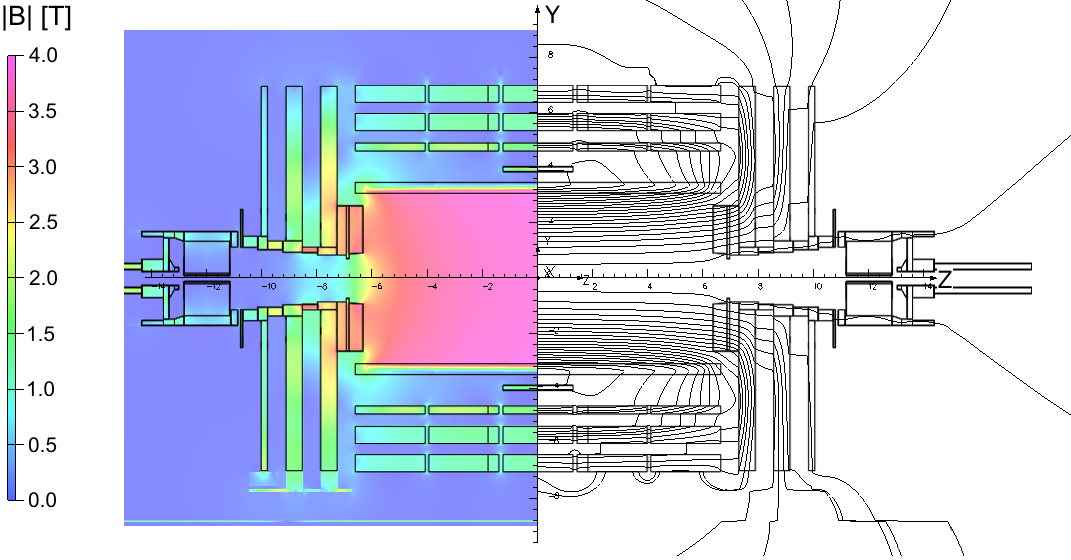
\includegraphics[width=0.8\linewidth]{Magnet.png}
    \caption{Value of $|B|$ (left) and field lines (right) predicted on a longitudinal section of the CMS detector, for the underground model at a central magnetic flux density of 3.8T. Each fieldline represents a magnetic flux increment of 6 Wb \cite{Chatrchyan:1215500}.}
    \label{fig:magnet}
\end{figure}
\indent Regarding the magnet, it is the largest solenoid superconducting magnet in the world. It consists of a cylinder 12.9 meters long, with an inner radius of 5.9 meters and an outer radius of 6.5 meters, which is wrapped with wire 2168 times \cite{Sphicas}. The electric current flowing through the wire creates a magnetic field of $3.8 \: T$ \footnote{Originally the solenoid was intended to produce a magnetic field of $4 \: T$ but in order to maximize its longevity, the operating field was reduced to $3. 8 \: T$ \cite{CMS_Collaboration_2010_4T}} (homogeneous inside the solenoid, see Figure \ref{fig:magnet}), about 100,000 times that of the Earth, while the total stored energy of the field reaches $2.3 \: GJ$, energy equivalent to about half a ton of TNT. To create a magnetic field of such a high intensity, an electric current of 18.164 kA is required, and to avoid the development of enormous temperatures due to this current intensity, the wire must be superconducting. In order to achieve superconductivity of the wire, it must be cooled to $-269^{\circ}$C.\\
\indent It is worth noting that the solenoid magnet is enclosed within 12-sided iron yokes 14 metres in diameter, which close the dynamic lines of the magnetic field coming out of the caps (so the magnetic field in the muon detector is in the opposite direction to that in the silicon detectors and calorimeters).The magnet together with the yokes weigh a total of 12500 tons making it the heaviest subsystem in the whole detector assembly.\\
\indent The magnetic field along the beam axis is parameterised as:
\begin{equation}
    B_z(0,z) = \frac{1}{2}B_0\sqrt{1+\Bar{a}}\cdot[f(u)+ f(v)]
\end{equation}
where
\begin{gather}
    u = (1-\Bar{z})/\Bar{a}, \: \: v= (1+\Bar{z})/\Bar{a} \nonumber\\
    \Bar{z} = 2z/L, \: \:  \Bar{a} = 2a/L \nonumber \\
    f(x) = x/\sqrt{1+x^2} \nonumber 
\end{gather}
with $a$ being the solenoid radius and $L$ its length.
Inside the solenoid region, the two components of the magnetic field (along the z axis and the radial one respectively) are parameterised as:
\begin{gather}
    B_z(r,z) = \sum_{\nu = 0}^{\infty} \frac{(-1)^{\nu}}{(\nu!)^2}\frac{\partial^{2\nu}}{\partial z^{2\nu}}B_z(0,z) \bigg(\frac{r}{2}\bigg)^{2\nu} \\
    B_r(r,z) = \sum_{\nu = 0}^{\infty} \frac{(-1)^{\nu}}{\nu!(\nu-1)!}\frac{\partial^{2\nu-1}}{\partial z^{2\nu-1}}B_z(0,z) \bigg(\frac{r}{2}\bigg)^{2\nu-1}
\end{gather}
\subsection{\label{sec:exp_CMS_5}The muon system}
\begin{figure}[htb!]
    \centering
    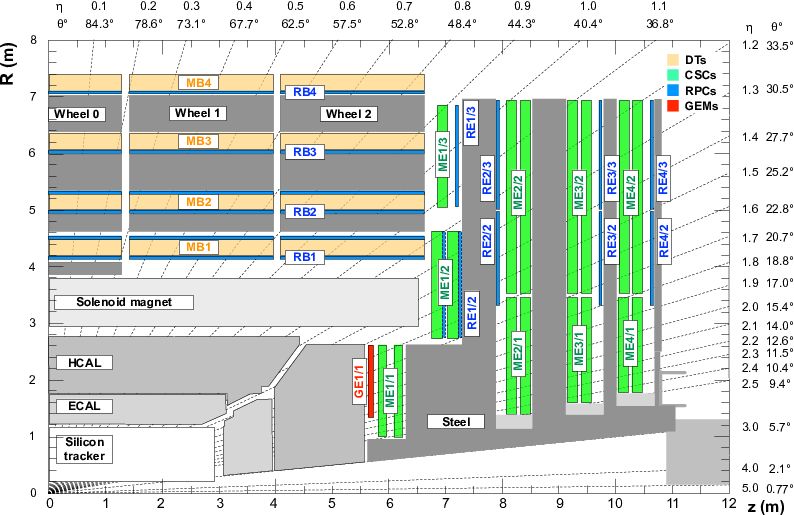
\includegraphics[width=0.9\linewidth]{Muon_system.png}
    \caption{Schematic view in the $r-z$ plane of a CMS detector quadrant \cite{Sirunyan_2018}.}
    \label{fig:Muon}
\end{figure}
\noindent The muon system \cite{Layter:343814, Sirunyan_2018} is located outside the solenoid magnet and comprises the outermost layer of the CMS detector. The objectives of the CMS muon system are to identify muons, measure their momenta, and provide signals for triggering on them. These goals are achieved with four complementary detector systems arranged in the steel flux-return yoke of the CMS solenoid. These subsystems are: the drift tubes (DTs), the cathode strip chambers (CSCs), the resistive-plate chambers (RPCs), and the recently added gas electron multiplier (GEM) detector. Altogether, the CMS muon detectors comprise almost one million electronic channels \cite{Hayrapetyan:2870088}.\\
\indent The physical arrangement of the muon detectors is shown in Fig. \ref{fig:Muon}. The central section is configured in a barrel geometry with four roughly cylindrical stations at different radii from the beam axis. The endcap section is arranged in four planar stations in z in each endcap.
\subsubsection{\label{subsubsec:exp_CMS_Muon_DTs}Drift Tubes}
\noindent The drift tube (DT) system in the barrel covers (fully) $|\eta| < 1.2 \: (0.83)$ and is composed of chambers formed by multiple layers of long rectangular tubes that are filled with an \ce{Ar} and \ce{CO2} gas mixture. An anode wire is located at the center of each tube, whereas cathode and field-shaping strips are positioned on its borders. They create an electric field that induces an almost uniform drift of ionization electrons produced by charged particles traversing the gas. The charged-particle trajectory is determined from the arrival time of the currents generated on the anode wires.

\subsubsection{\label{subsubsec:exp_CMS_Muon_CSCs}Cathode Strip Chambers}
\noindent The cathode strip chamber (CSC) system in the endcap comprises multiwire proportional chambers having cathode strips with an $R-\phi$ geometry and covering (fully) the region $0.9 \: (1.24) < |\eta| < 2.4$ . The CSCs are operated with a gas mixture of \ce{Ar}, \ce{CO2}, and \ce{CF4}. Signals are generated on both anode wires and cathode strips. The finely segmented cathode strips and fast readout electronics provide good timing and spatial resolution to trigger on and identify muons. Because of the higher flux of particles in the endcap region, the CSCs are designed to have a faster response time than the DTs.

\subsubsection{\label{subsubsec:exp_CMS_Muon_RPCs}Resistive Plate Chambers}
\noindent The RPCs are located in both the barrel and endcap regions, and they complement the DTs and CSCs with a very fast response time that can be used to unambiguously identify the bunch crossing corresponding to a muon trigger candidate. The RPCs comprise two detecting layers of high-pressure laminate plates that are separated by a thin gap filled with a gas mixture of \ce{C2H2F4}, \ce{i-C4H10}, and \ce{SF6}. The electronic readout strips are located between the two layers, and the high voltage is applied to high-conductivity electrodes coated on each plate. The detectors are operated in avalanche mode to cope with the high background rates.

\subsubsection{\label{subsubsec:exp_CMS_Muon_GEMS}Gas Electron Multiplier}
\noindent To enhance the track reconstruction and trigger capabilities of the endcap muon spectrometer, large-area triple-layer gas electron multiplier (GEM) detectors \cite{SAULI1997531} were installed in the region covering $1.55 < |\eta| < 2.18$ of the CMS detector for the Run 3. The first station, denoted GE1/1, was installed at the very start of Run 3 while the second station, GE2/1 was added during the Year End Technical Stop (YETS) in 2024.  \\
\indent The key feature of the GEM is a foil consisting of a perforated insulating polymer surrounded on the top and bottom by conductors. A voltage difference is applied on the foils producing a strong electric field in the holes. The GEM is operated with a gas mixture of \ce{Ar} and \ce{CO2}. When the gas volume is ionized, electrons are accelerated through the holes and read out on thinly separated strips. This structure allows for high amplification factors with modest voltages that provide good timing and spatial resolution, and can be operated at high rates.
%Figure 39 shows a quadrant of the CMS detector with the location of the GE1/1 highlighted and outlined in red in the r–z plane. A detailed drawing is shown in Fig. 73.

\subsection{\label{sec:exp_CMS_6}Forward detectors}

\subsubsection{\label{subsubsec:exp_CMS_CASTOR}CASTOR Calorimeter}
\noindent The CASTOR (Centauro And Strange Object Research) calorimeter \cite{gunnellini2013castor, roland2010forward, CMS:2020ldm}, is located 14.37 m from the CMS interaction point and extends the forward rapidity coverage to the region $-6.6 < \eta < -5.2$ \footnote{Only on the negative longitudinal side of CMS}. CASTOR is a sampling electromagnetic and hadronic calorimeter and presents a sandwich structure of tungsten (W) absorber plates and quartz plates as active material. The collection of the signal is based on the production of Cerenkov photons which are transmitted to photomultiplier tubes through aircore lightguides. The tungsten and quartz plates are inclined by $45^\circ$ with respect to the beam axis to optimize the photon yield (Figure \ref{fig:CASTOR}).
\begin{figure}[H]
    \centering
    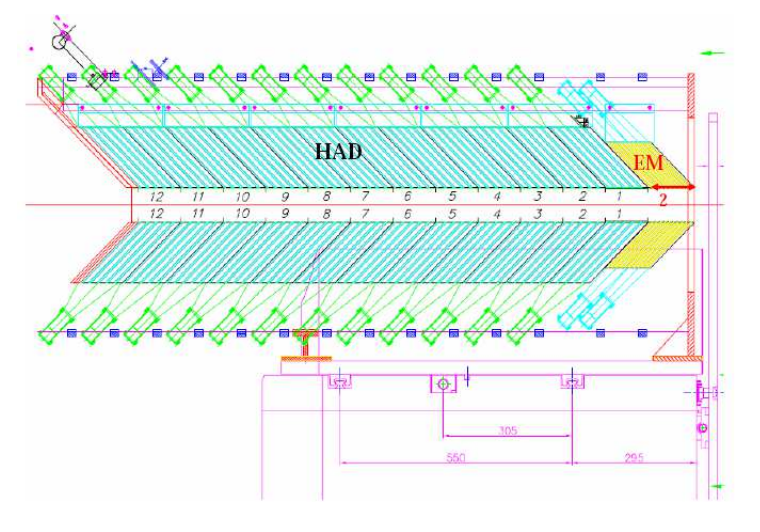
\includegraphics[width=0.55\linewidth]{CASTOR.png}
    \caption{The CASTOR calorimeter \cite{roland2010forward}.}
    \label{fig:CASTOR}
\end{figure}
\subsubsection{\label{subsubsec:exp_CMS_ZDC} Zero Degree Calorimeter}
\noindent The Zero Degree Calorimeter (ZDC) \cite{roland2010forward} detects neutral particles in $|\eta| > 8.5$ region. These detectors are located at $z = \pm 140\: m$ from the interaction point. The CMS ZDC is able to measure the spectator neutron multiplicity distribution. Its fibres are made up of quartz, its effective material is tungsten, and its technology is similar with that of the CASTOR calorimeter.
\subsection{\label{sec:exp_CMS_7}Triggering system}

\noindent The LHC collides proton bunches at a rate of 40 MHz, spaced 25 ns apart. Considering a storage size of $\sim $ 1 MB per bunch crossing event, the LHC collision frequency would result to data output of 40 TB per second, which is unfeasible to be recorded. However, not all collision events hold pertinent information for physics investigations. Hence, a meticulous selection process is necessary to isolate events of interest while discarding the rest. To accomplish this, the CMS employs a sophisticated two-tiered trigger system: the Level-1 Trigger (L1 Trigger), implemented in hardware and the High-Level Trigger (HLT), implemented in software.
\subsubsection{\label{sec:exp_CMS_trigger_1} Level-1 Trigger}
\noindent The L1 Trigger system is instrumented with custom-designed hardware processors, and runs event selection algorithms using information from the CMS subdetectors. It takes a decision within 3.8 $\mu$s and selects up to 110 kHz of interesting events, out of the 40 MHz rate it receives.\\
\indent The L1 Trigger consists of two primary components: the L1 calorimeter trigger and the L1 muon trigger. The output of the two subsystems is collected by the Global Trigger (GT) which takes the final decision on the event. The decision is made based on approximately 500 event selection algorithms that depend on kinematic quantities, position, isolation and quality of the event’s objects. The selection algorithms, also referred to as L1 Trigger seeds, are executed in parallel for the final trigger decision. A schematic representation of the CMS L1 Trigger structure is depicted in Figure \ref{fig:L1T}.\\
\begin{figure}[H]
    \centering
    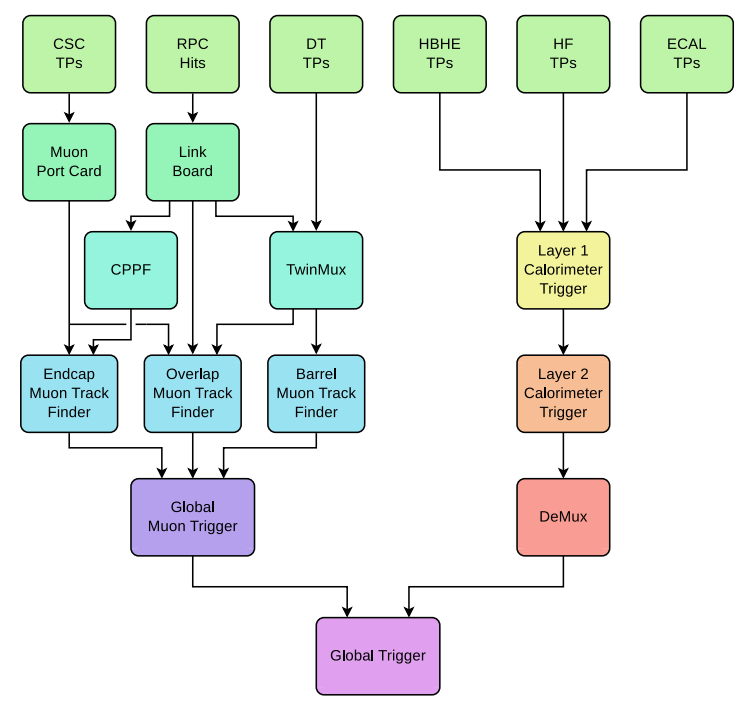
\includegraphics[width=0.78\linewidth]{L1T.png}
    \caption{Diagram of the CMS L1 Trigger system \cite{Sirunyan_2020}}
    \label{fig:L1T}
\end{figure}
\indent The L1 Calorimeter Trigger consists of two layers. The Layer-1 receives, calibrates and sorts the local energy deposits, which are called "trigger primitives" (TP) and are sent from ECAL, HCAL and HF. The Layer-2 uses the TPs to reconstruct physics objects. The input to Layer-1 is organized into trigger towers (TT) that correspond to $\Delta\eta \times\Delta\phi$ of $0.087 \times 0.087$ each. Every TT encodes energy deposits at a specific position in the calorimeters. A Time Multiplexed Trigger (TMT) architecture is used and allows for the information of all the TT in the event to be received by the Layer-2. There are no regional boundaries in the object reconstruction and the full granularity is exploited when the energy deposits are computed. The output of the TMT nodes are collected in the de-multiplexing (DeMux) node, sorted and sent to GT \cite{M_Baber_2014}. The calorimeter trigger creates two different types of trigger object, reflecting the two fundamental types of energy deposition in the calorimeter; electron/photon candidates and jets. The former are spatially-compact objects mainly confined to the ECAL, while the latter are larger and primarily in the HCAL. In addition, algorithms have been developed aiming at reconstructing efficiently hadronically decaying $\tau$ leptons using the combination of the ECAL and HCAL energies, thus creating possible $\tau$ candidates \cite{Zabi_2016}.

The L1 muon trigger consists of three regional muon reconstructing algorithms \cite{Fulcher:2302108,Jeitler:2165960}:
\begin{itemize}
    \item The Barrel Muon Track Finder (BMTF) receives DT TPs and RPC hits from $|\eta| < 0.83$. The TPs and hits are combined in “superprimitives” in TwinMux
    \item The Overlap Muon Track Finder (OMTF) receives uncombined DT TPs and RPC hits transmitted from TwinMux, together with CSC TPs. The TPs and hits delivered to the OMTF cover the range from $0.83 < |\eta| < 1.24$
    \item The Endcap Muon Track Finder (EMTF): takes as input CSC TPs and RPC hits from the forward pseudorapidity regions of $1.24 < |\eta| < 2.4$, through CPPF (Concentration Preprocessing and Fan-out).
\end{itemize}
\indent The muon track finder algorithms measure the charge, transverse momentum and bending angle of the L1 muon candidates, and assign to them a quality bit based on the reconstruction fit. Upon receiving up to 36 L1 muon candidates from each track finder, the GMT undertakes several tasks to refine the selection. Firstly, it sorts the candidates by transverse momentum and assesses their quality based on parameters such as pT resolution and hit count, while eliminating duplicate entries. Furthermore, the GMT incorporates spatial coordinates from the muon stations, extrapolating each candidate's track back to the interaction point. The extrapolation corrections are derived from simulation as a function of $p_{T} , \eta, \phi$ and charge and are stored in look up tables (LUT). The corrected coordinates are propagated to the GT and improve the performance of the L1 trigger seeds that rely on the invariant mass or the spatial coordinate difference between multiple muons.\\
\indent A maximum of 8 muon candidates are chosen based on a combination of quality and transverse momentum metric and are sent to the GT for the final L1 Trigger decision. The GT collects L1 muons and calorimeter objects and executes every selection algorithm in parallel in order to make the final trigger decision.

\subsubsection{\label{sec:exp_CMS_trigger_2}High Level Trigger and Data Acquisition}
\noindent The HLT task is to further reduce the event rate to 1 kHz. To achieve this, all events that pass the L1 Trigger are sent to a computer farm of approximately 30k CPU cores, known as the Event Filter Farm. This is located in a dedicated room at the surface of the CMS cavern. The HLT has access to the full detector readout, including the tracker information, and runs a lighter version of the offline event reconstruction.\\
\indent An important concept of the HLT data processing is the "path", which is a set of algorithm steps, running in predefined order, both for reconstruction of physics objects and for selection. Each path is a sequence of steps of increasing complexity. If an event is accepted by at least one path it is stored, otherwise it is discarded.\\
\indent Events accepted by the HLT are transferred to another software process called the storage manager, under the supervision of the Data Acquisition system (DAQ). The data events are first stored locally on disk, into multiple primary datasets (PD). Each PD is fed by a number of logically coherent trigger paths. When operating, CMS records about 80 TB of data every day, which corresponds to approximately $ 80 \times 120 \sim 9.6$ PB per run period. The recorded events are reconstructed with offline algorithms and the post-processing results are stored in NanoAOD format based on the ROOT framework \cite{Peruzzi_2020}. A world wide computing farm with three-tier structure is used for the processing and storage of the data.

\section{\label{sec:exp_CMS_8}The L1 muon trigger performance}
\noindent The most important metric of a triggering system is its efficiency, i.e. the fraction of events the trigger was supposed to collect to the fraction of events which is really collected. In order to perform an efficiency measurement without using a separate reference trigger, leading to almost unbiased estimates, a technique called tag-and-probe is used \cite{Muon_2012}. In this method, both the "tag" muon and the "probe" muon are selected using the same strict criteria, with the exception that the tag muon is specifically required to have fired the HLT. This ensures that the selection applied to the probe muon does not introduce bias into the efficiency measurement. The fraction of probe muons that passes the selection under study gives an estimate of its efficiency.
\begin{equation}
    \epsilon_{probe} = \frac{N_{pass}^{tag\&probe}}{N_{pass}^{tag}}
\end{equation}
Basically, the tag muon always fires the trigger, independently of the probe, while the probe muon fires the trigger only in some cases, thus giving us the unbiased trigger efficiency.\\
\indent The efficiency of the L1 muon trigger was measured in data with this tag-and-probe technique using offline reconstructed muons from $Z \rightarrow \mu\mu$ events. Figures \ref{subfig:eff_pt} and \ref{subfig:eff_pt2} show the efficiency as a function of the reconstructed probe muon $p_T$, for a L1 $p_T$ threshold of 22 GeV, for the four different $\eta$ regions: BMTF, OMTF, EMTF as well as the inclusive region, GMT. The inclusive in $\eta$ efficiency is higher than 90\% for the specific L1 $p_T$ threshold and it reaches 93\% at the plateau.
\begin{figure}[H]
    \centering
    \begin{subfigure}{0.48\textwidth}
        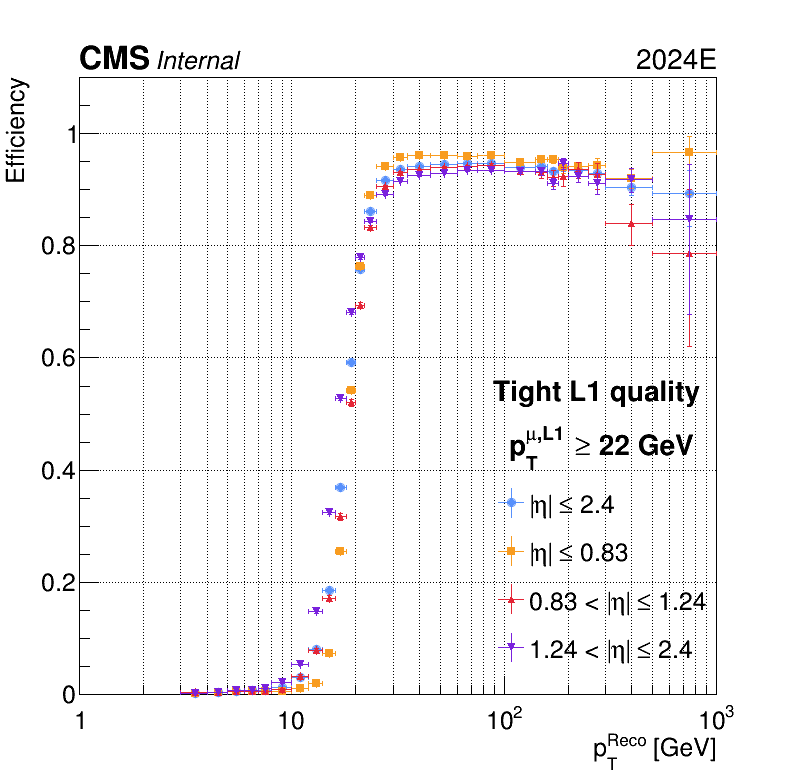
\includegraphics[width =1.0\linewidth]{eff_SingleMu_22_pt.png}
        \caption{}
        \label{subfig:eff_pt}
    \end{subfigure}
    \begin{subfigure}{0.48\textwidth}
        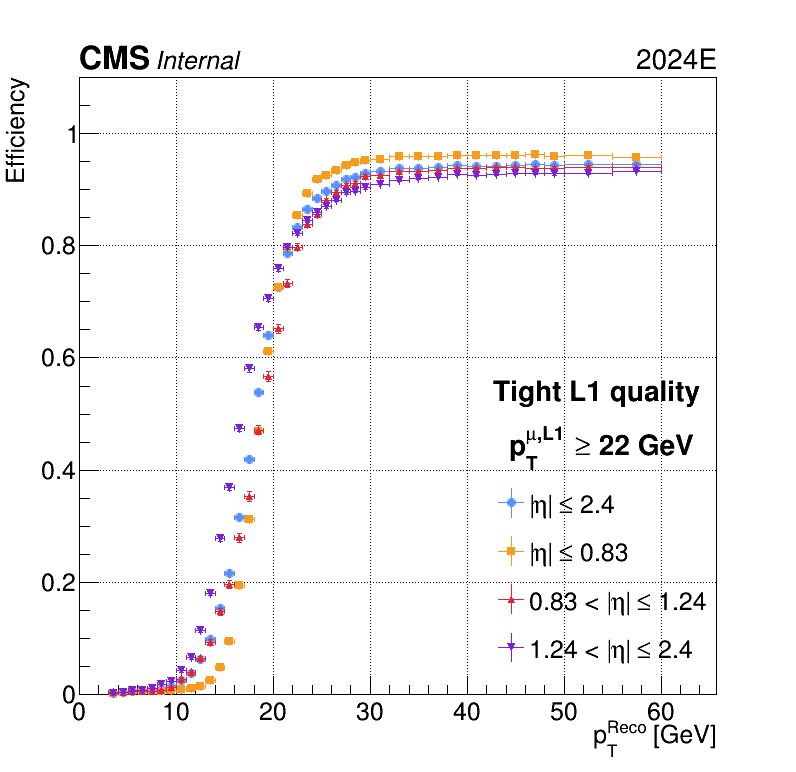
\includegraphics[width =1.0\linewidth]{eff_SingleMu_22_pt2.png}
        \caption{}
        \label{subfig:eff_pt2}        
    \end{subfigure} 
    \caption{The single-muon L1 Trigger efficiency for 2024 data as a function of probe muon $p_T$}
    \label{fig:eff_pt}
\end{figure}
\begin{figure}[H]
    \centering
    \begin{subfigure}{0.48\textwidth}
        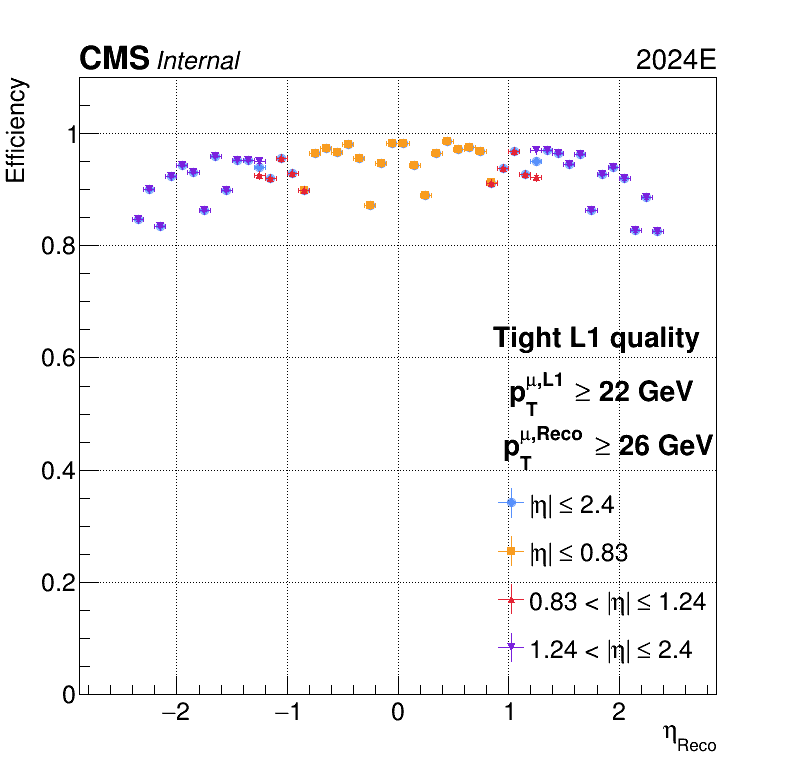
\includegraphics[width =1.0\linewidth]{eff_SingleMu_22_eta.png}
        \caption{}
        \label{subfig:eff_eta}
    \end{subfigure}
    \begin{subfigure}{0.48\textwidth}
        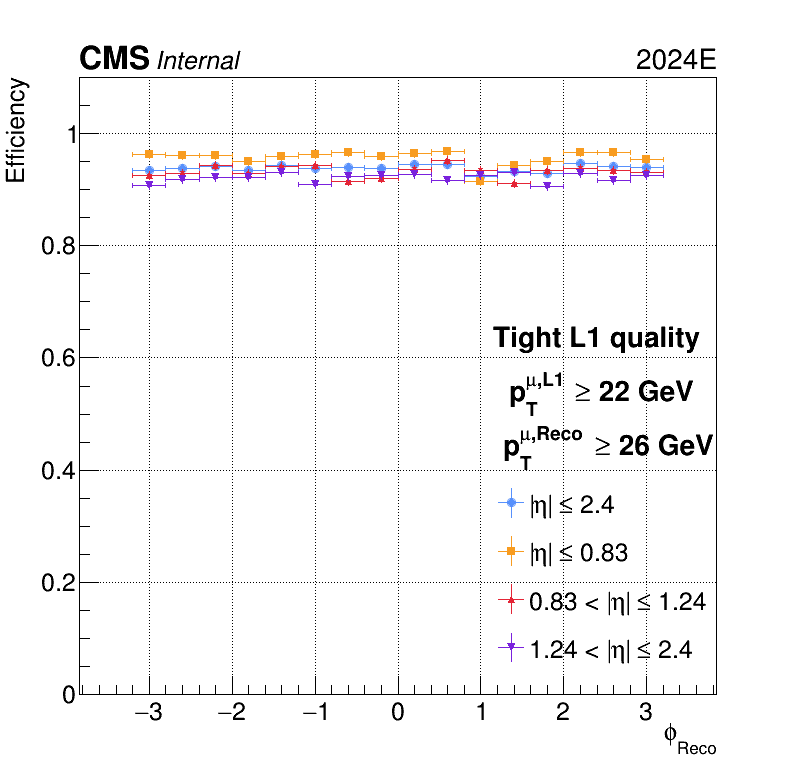
\includegraphics[width =1.0\linewidth]{eff_SingleMu_22_phi.png}
        \caption{}
        \label{subfig:eff_phi}        
    \end{subfigure} 
    \caption{The single-muon L1 Trigger efficiency for 2024 data as a function of probe muon (a) $\eta$ and (b) $\phi$}
    \label{fig:eff_eta&phi}
\end{figure}

Among the three regional track finders, it is easy to see that the BMTF has the best efficiency, while EMTF has the worst. This can be seen better in Figure \ref{subfig:eff_eta} where the efficiency as a function of the reconstructed probe muon $\eta$ is illustrated. From this plot, it is obvious that, the efficiency is consistently above 95\%, with the exception of two points. These drops are due to the gaps between the central DT "wheel" (Wheel 0) and the neighboring wheels (Wheels 1 \& -1), where muons passing through these gaps do not leave enough hits in the DTs and thus they are often not reconstructed (see Figure \ref{fig:Muon}).
%These are the points where the optical links are connected to the detector, resulting in the drop of the efficiency. 
As far as the EMTF, we can see that while we go outwards, towards bigger $|\eta|$ the efficiency drops significantly, reaching as low as 80\%. This efficiency drop, originates from the inhomogenous and weaker magnetic field (CSCs are located outside the magnet) and the higher occupancy of the chambers in the forward directions.\\
\indent For completeness, in Figure \ref{subfig:eff_phi} the efficiency as a function of the reconstructed probe muon $\phi$ is presented. We can see that for the region around $\phi = 1$ there is a small drop in efficiency for all $\eta$ regions. This is caused by the so-called "chimney", the vertical-pit where readout fibers go from the detector to the surface and opens a hole in the DT (and GMT) system. The EMTF and OMTF efficiencies should not have this feature. This effect is better illustrated in Figure \ref{fig:eff_eta_phi}, where a two dimensional plot representing the efficiency in the whole coverage of the detector is presented.
\begin{figure}[H]
    \centering
    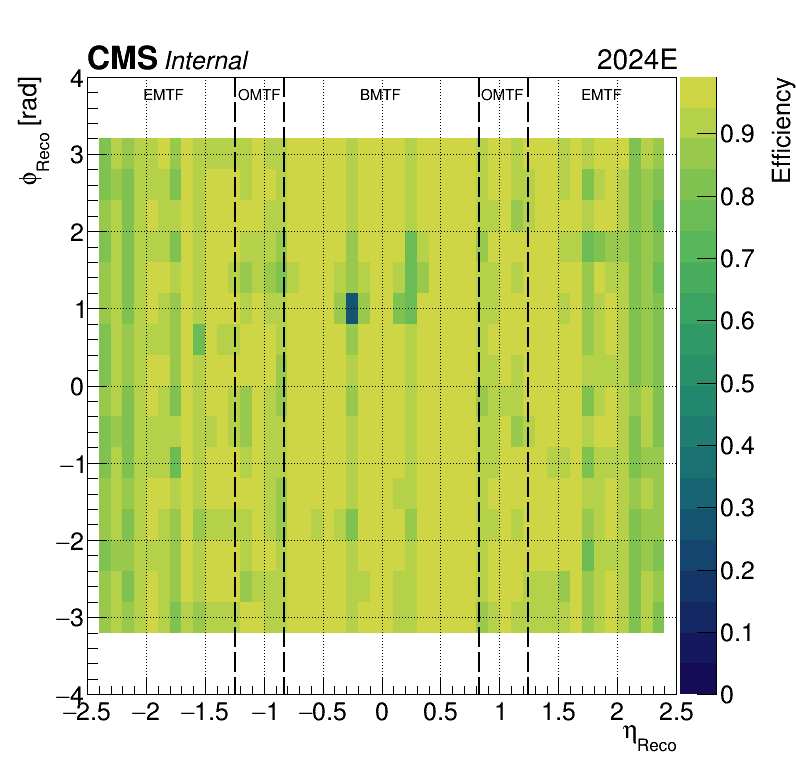
\includegraphics[width =0.6\linewidth]{eff_SingleMu_22_phi_eta.png}
    \caption{Heatmap of the single-muon L1 Trigger efficiency for 2024 data}
    \label{fig:eff_eta_phi}
\end{figure}
\indent Another important metric of the triggering system is the charge misidentification probability. This basically, indicates, how good the reconstruction is between the L1 and offline muons. In contrast with the calculation of the efficiency, for the charge misidentification probability we do not use the tag-and-probe method, but we simply match the L1 muons with the corresponding reconstructed muons and compare the charges between the two. The results are shown in Figure \ref{fig:misid_pt} as a function of the reconstructed probe muon $p_T$, for a L1 $p_T$ threshold of 22 GeV, for the four different $\eta$ regions. In Figure \ref{fig:misid_eta_phi}, the two dimensional plot representing the charge misidentification probability in the whole coverage of the detector is presented.

\begin{figure}[H]
    \centering
    \begin{subfigure}{0.48\textwidth}
        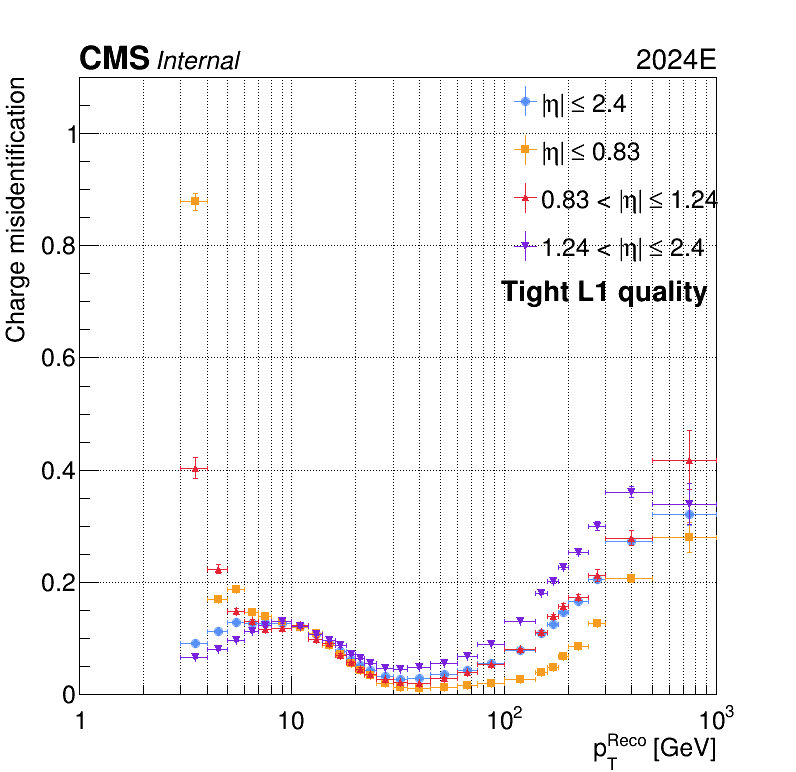
\includegraphics[width =1.0\linewidth]{misid_pt.png}
        \caption{}
        \label{subfig:misid_pt}
    \end{subfigure}
    \begin{subfigure}{0.48\textwidth}
        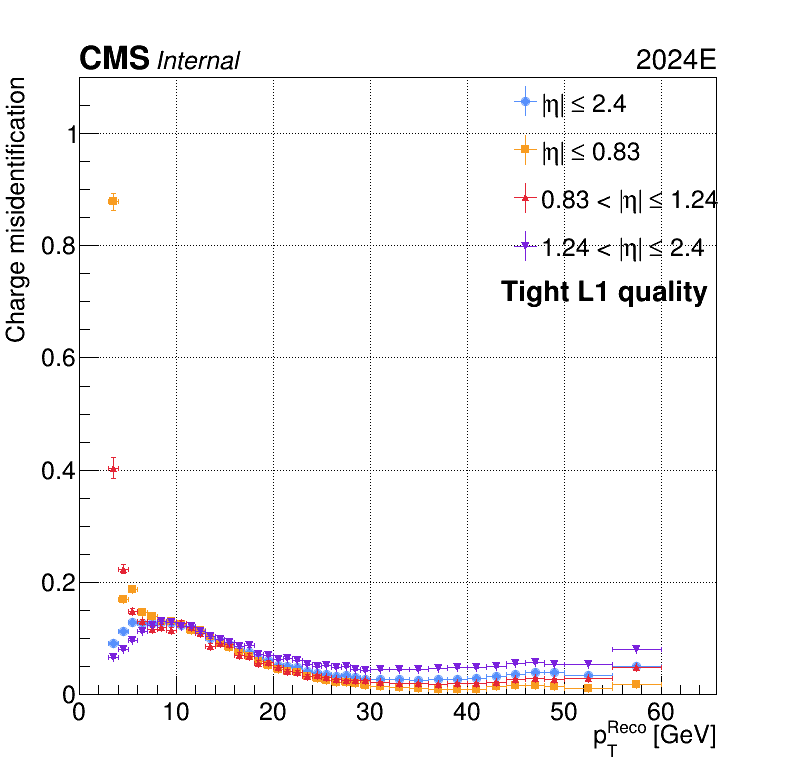
\includegraphics[width =1.0\linewidth]{misid_pt2.png}
        \caption{}
        \label{subfig:misid_pt2}        
    \end{subfigure} 
    \caption{The charge misidentification for 2024 data as a function of the reconstructed muon $p_T$}
    \label{fig:misid_pt}
\end{figure}

\begin{figure}[H]
    \centering
    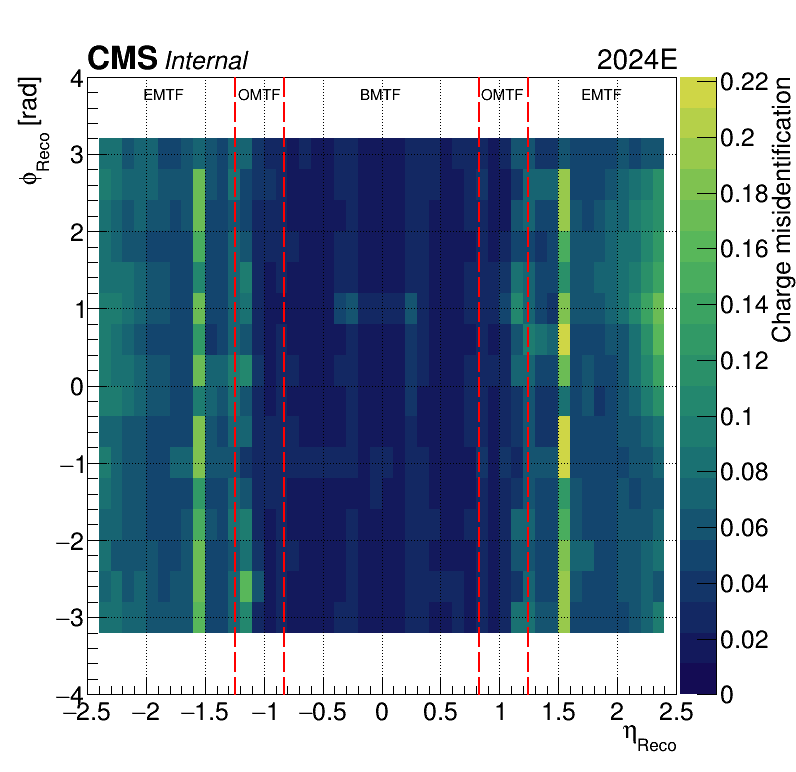
\includegraphics[width =0.6\linewidth]{misid__phi_eta.png}
    \caption{Heatmap of the charge misidentification for 2024 data}
    \label{fig:misid_eta_phi}
\end{figure}
